\section{RESULTADOS DA EXECUÇÃO DE EXPERIMENTOS COMPUTACIONAIS}
\label{sec:resultados}

% \subsection{Teste 0001}
% 
% Em sequência são apresentados os parâmetros utilizados e resultados obtidos com a execução do teste denominado \textit{0001}. Utilizou-se o ambiente de Cascavel/PR com $286.205$ agentes. A população de agentes foi definida com base nos dados populacionais de 2010 disponibilizados pelo IBGE, que estratifica a população por faixas etárias e sexo, como ilustrado na Tabela \ref{tab:populacoes_0001}. O consumo de memória da simulação permaneceu em torno de $3,278$MB e o tempo de execução foi de $87,47$s. \\
% 
% \begin{table}[H]
% \centering
% \begin{tabular}{c|c|c|c}
%  \textbf{Faixa Etária} 		& \textbf{Sexo Masculino}	& \textbf{Sexo Feminino}	& \textbf{Total}	\\ \hline
%   Criança			& $33.029$			& $32.029$			& $65.058$		\\
%   Jovem				& $27.508$			& $27.144$			& $54.652$		\\
%   Adulto			& $67.768$			& $73.023$			& $140.791$		\\
%   Idoso				& $11.466$			& $14.238$ 			& $25.704$		\\ \hline
%   \textbf{Total}		& $139.771$			& $146.434$			& $286.205$		\\
% \end{tabular}
% \caption{Tabela das populações de agentes por faixas etárias e sexos, baseada nos dados disponibilizados pelo IBGE.}
% \label{tab:populacoes_0001}
% \end{table}
% 
% \newpage
% 
% \textbf{Arquivo Geral.csv:} 
% 
% \begin{center}
% \pgfplotstabletypeset[
% col sep = semicolon,
% every head row/.style={before row=\toprule,after row=\midrule},
% every last row/.style={after row=\bottomrule},
% display columns/2/.style={string type, column type=l}
% ]{Figuras/Resultados/0001/Entradas/MonteCarlo_0/Geral.csv}
% \end{center}
% 
% \newpage
% 
% \subsubsection{Quantidades de Agentes Infectados Acumulados ao Longo do Tempo de Simulação}
% 
% A Figura \ref{fig:Quantidades_Agentes_Infectados_Acumulado_0001} ilustra as quantidades de agentes infectados acumulados.
% 
% \begin{figure}[H]
%   \centering
%   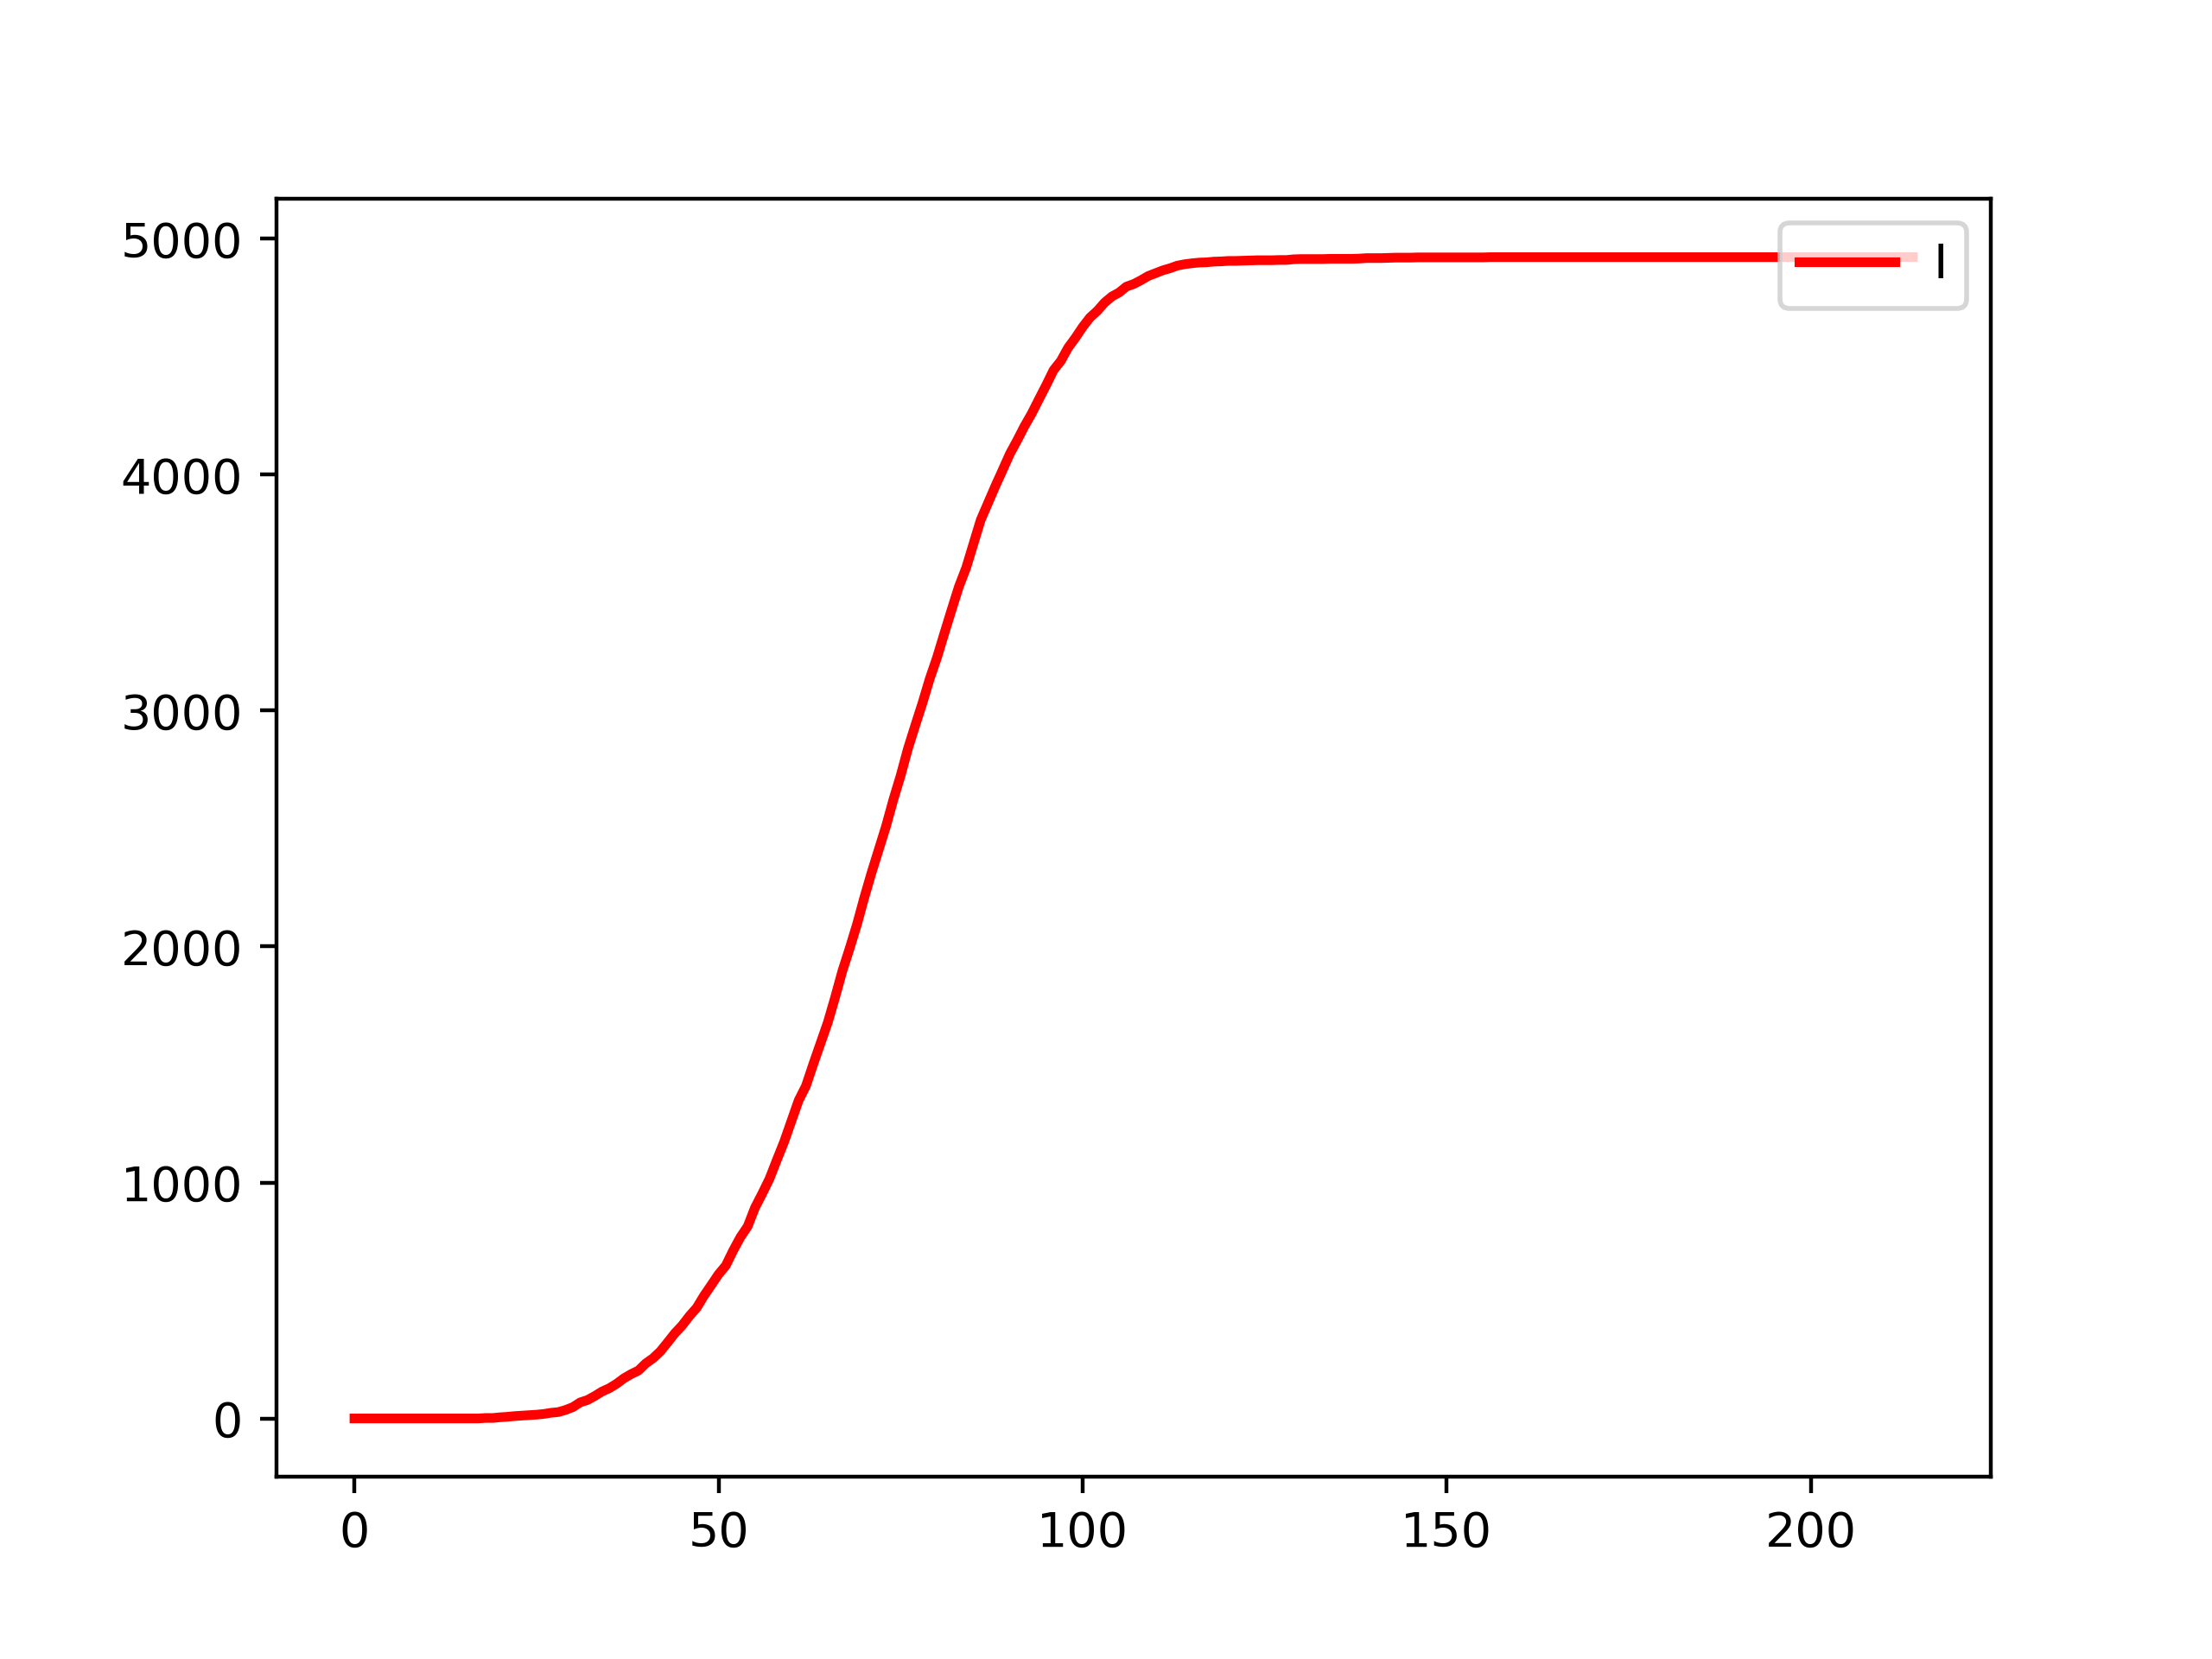
\includegraphics[width=1.0\textwidth]{Figuras/Resultados/0001/Saidas_GPU_BIT/MonteCarlo_0/Quantidades_Novo_Total_Acumulado_Total.png}
%   \caption{Quantidades de agentes infectados acumulados.}
%   \label{fig:Quantidades_Agentes_Infectados_Acumulado_0001}
% \end{figure}
% 
% A Figura \ref{fig:Casos_Observados_Acumulados_0001} ilustra as quantidades de casos observados acumulados.
% 
% \begin{figure}[H]
%   \centering
%   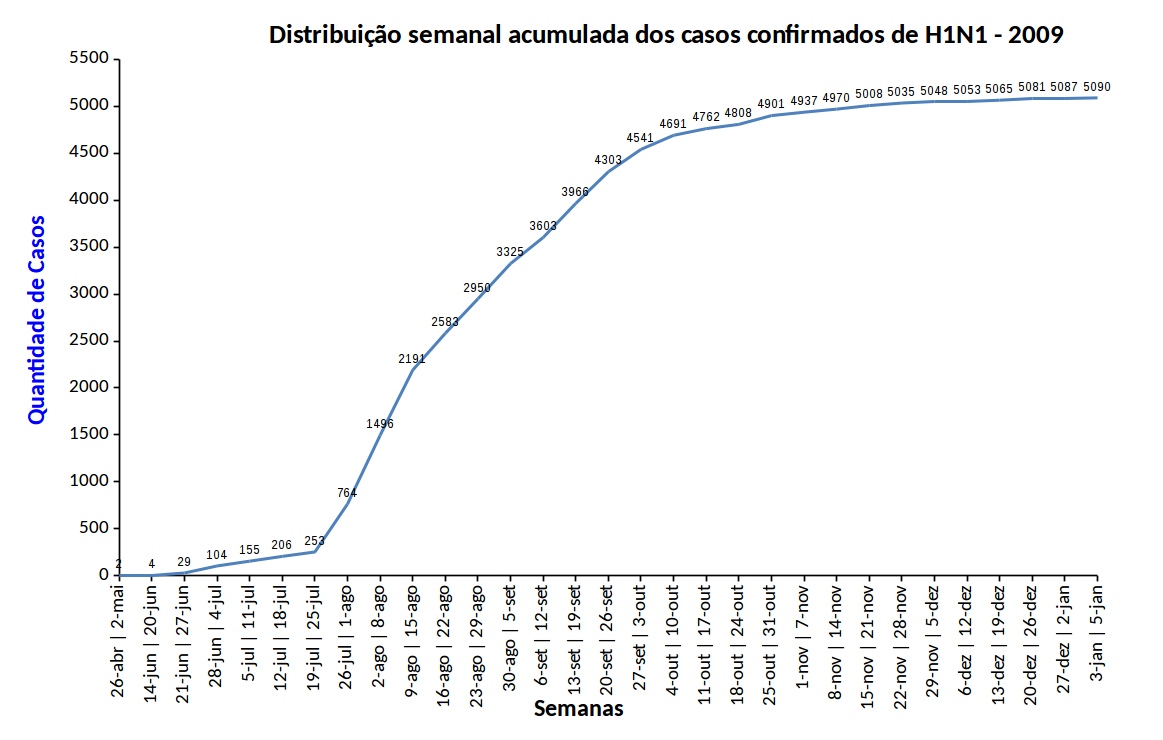
\includegraphics[width=1.0\textwidth]{Figuras/Resultados/Observado/Casos_Observados_Acumulados.png}
%   \caption{Quantidades de casos observados acumulados.}
%   \label{fig:Casos_Observados_Acumulados_0001}
% \end{figure}
% 
% \newpage
% 
% \subsubsection{Espalhamento Espacial dos Casos de Influenza ao Longo do Tempo de Simulação}
% 
% A Figura \ref{fig:casos_0001} ilustra o espalhamento espacial dos casos de Influenza no ambiente nos ciclos 1, 40, 80, 120, 160 e 200.
% 
% \begin{figure}[H]
%   \centering
%   \begin{minipage}{.5\textwidth}
%     \centering
%     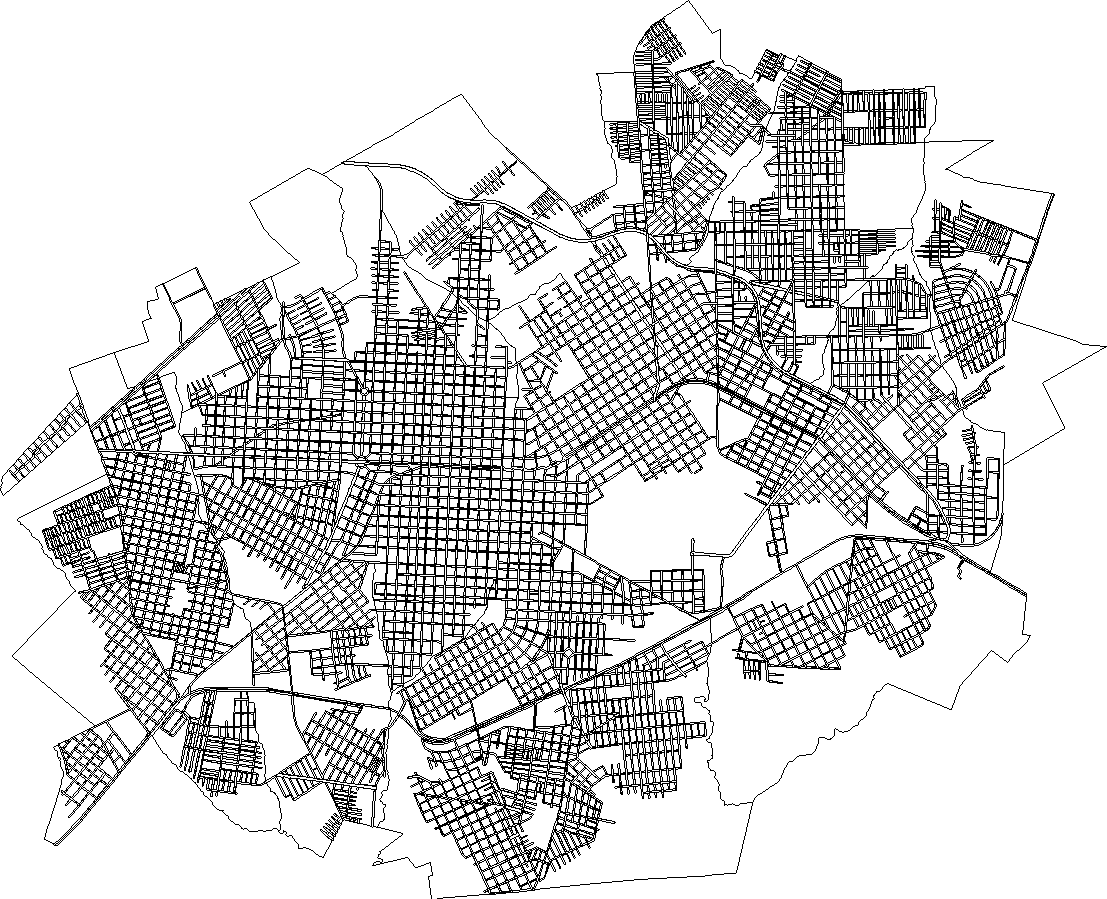
\includegraphics[width=1.0\textwidth]{Figuras/Resultados/0001/Saidas_GPU_BIT/MonteCarlo_0/Simulacao_0/Casos/00000.png}
%     \captionsetup{labelformat=empty}
%     \captionof{figure}{Ciclo 1}
%   \end{minipage}%
%   \begin{minipage}{.5\textwidth}
%     \centering
%     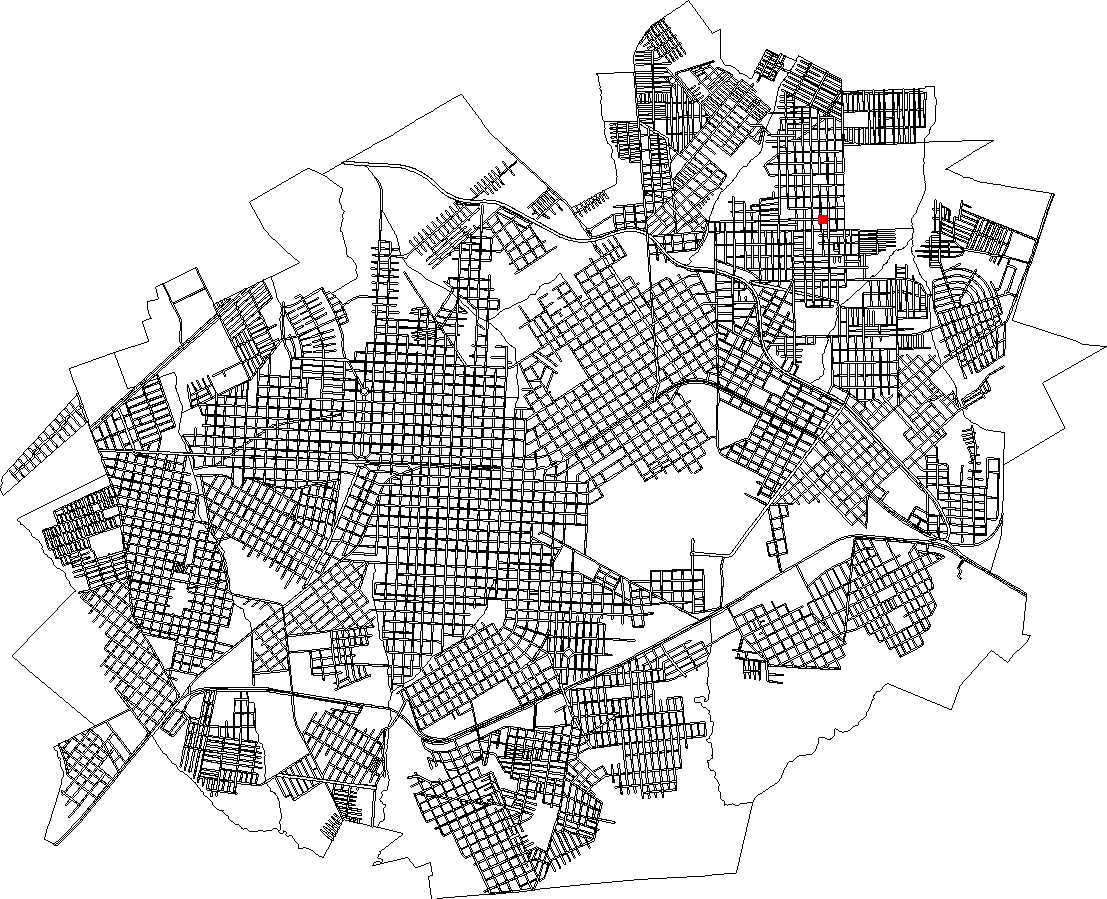
\includegraphics[width=1.0\textwidth]{Figuras/Resultados/0001/Saidas_GPU_BIT/MonteCarlo_0/Simulacao_0/Casos/00040.png}
%     \captionsetup{labelformat=empty}
%     \captionof{figure}{Ciclo 40}
%   \end{minipage}
%   \begin{minipage}{.5\textwidth}
%     \centering
%     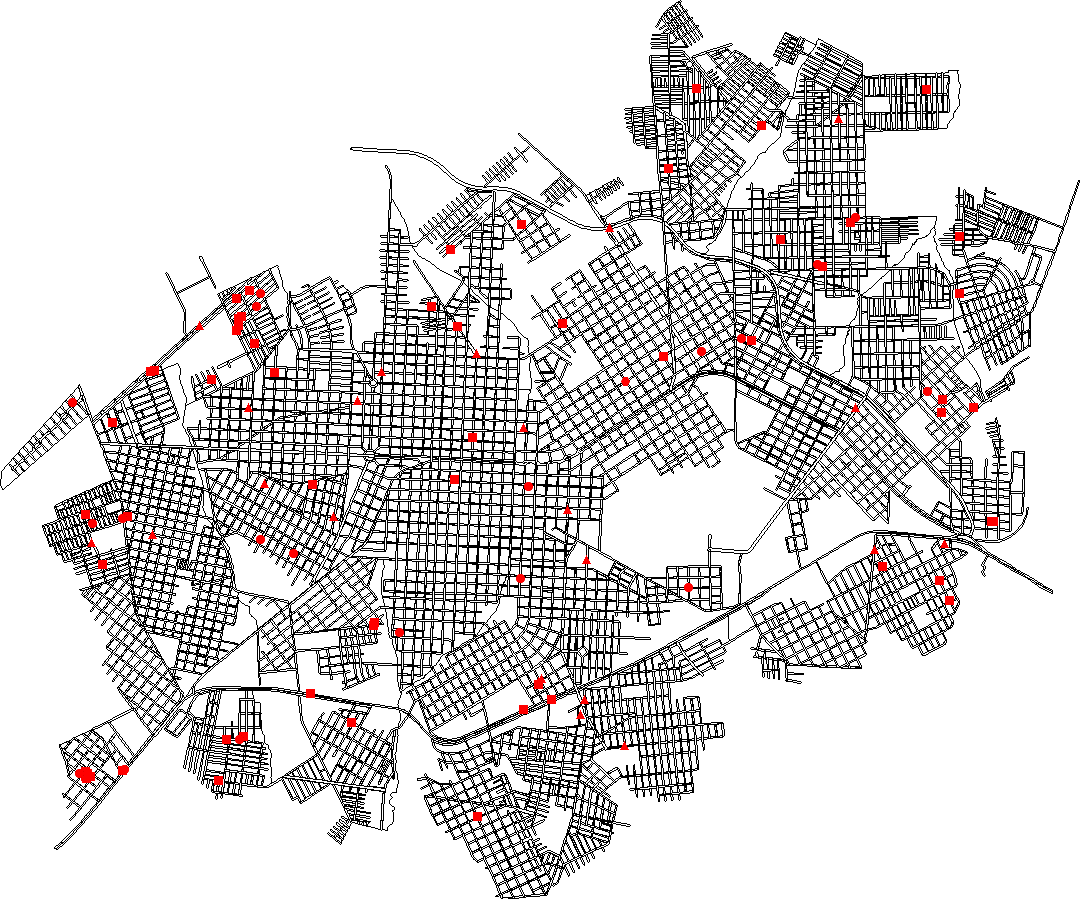
\includegraphics[width=1.0\textwidth]{Figuras/Resultados/0001/Saidas_GPU_BIT/MonteCarlo_0/Simulacao_0/Casos/00080.png}
%     \captionsetup{labelformat=empty}
%     \captionof{figure}{Ciclo 80}
%   \end{minipage}%
%   \centering
%   \begin{minipage}{.5\textwidth}
%     \centering
%     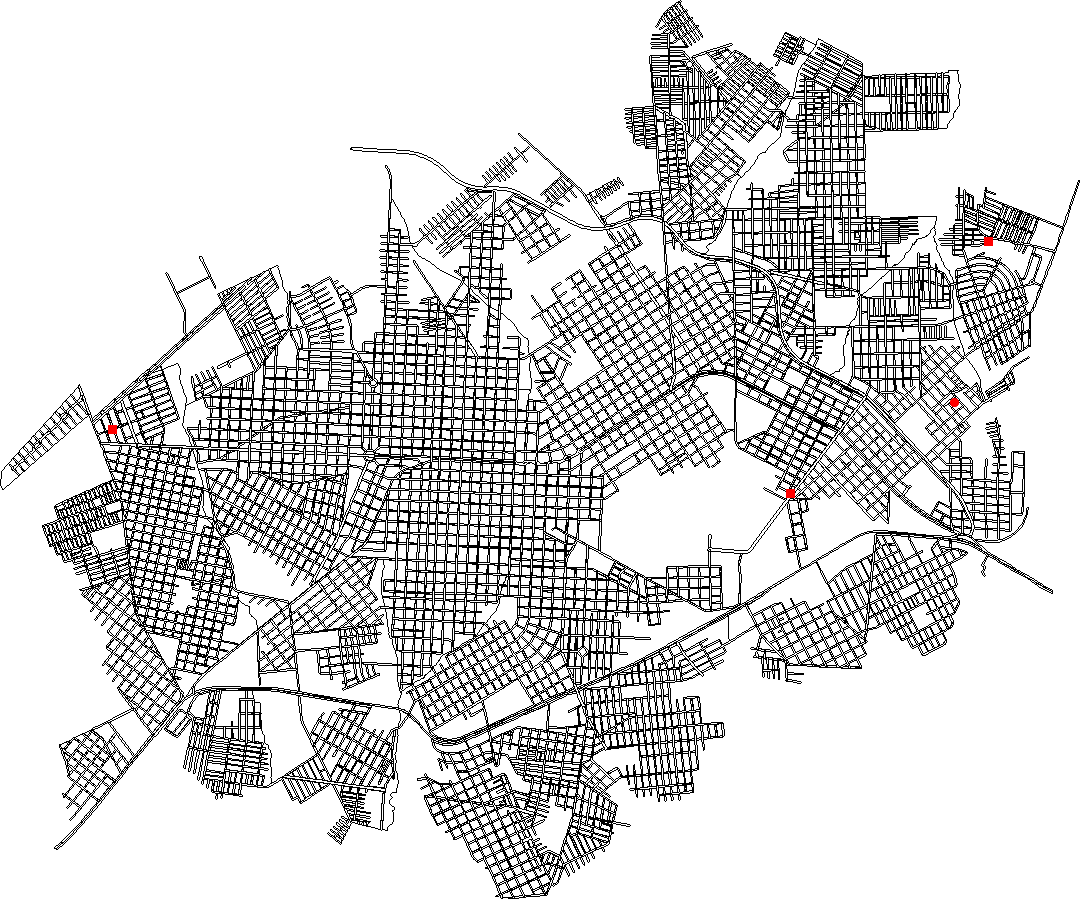
\includegraphics[width=1.0\textwidth]{Figuras/Resultados/0001/Saidas_GPU_BIT/MonteCarlo_0/Simulacao_0/Casos/00120.png}
%     \captionsetup{labelformat=empty}
%     \captionof{figure}{Ciclo 120}
%   \end{minipage}
%   \begin{minipage}{.5\textwidth}
%     \centering
%     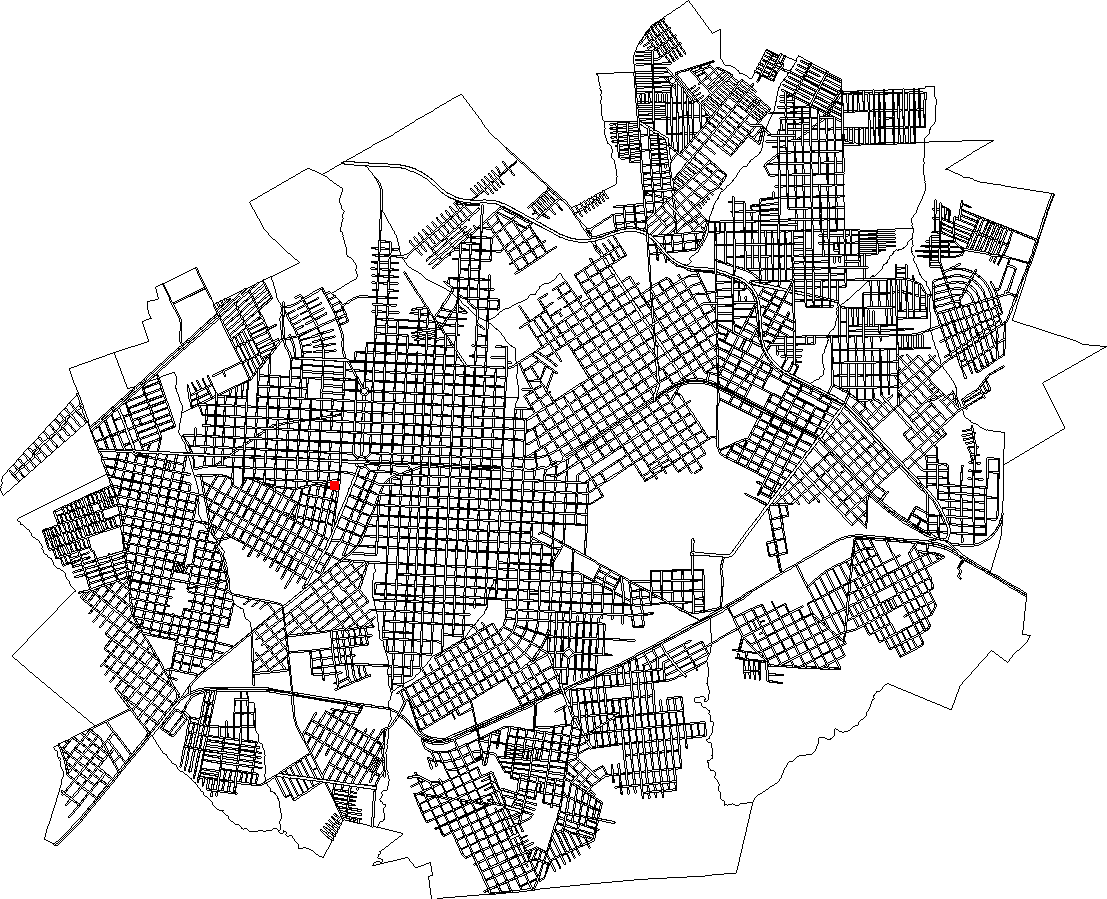
\includegraphics[width=1.0\textwidth]{Figuras/Resultados/0001/Saidas_GPU_BIT/MonteCarlo_0/Simulacao_0/Casos/00160.png}
%     \captionsetup{labelformat=empty}
%     \captionof{figure}{Ciclo 160}
%   \end{minipage}%
%   \begin{minipage}{.5\textwidth}
%     \centering
%     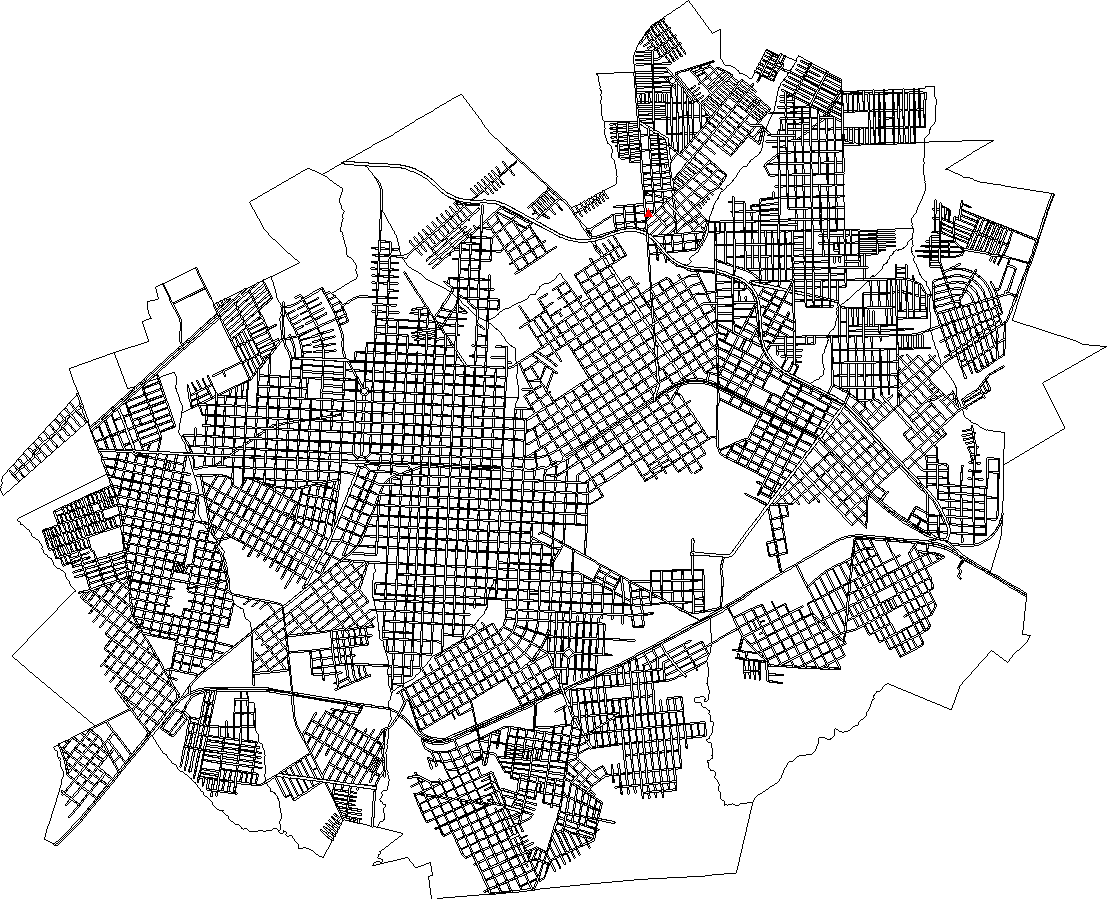
\includegraphics[width=1.0\textwidth]{Figuras/Resultados/0001/Saidas_GPU_BIT/MonteCarlo_0/Simulacao_0/Casos/00200.png}
%     \captionsetup{labelformat=empty}
%     \captionof{figure}{Ciclo 200}
%   \end{minipage}
%   \caption{Espalhamento espacial dos casos de Influenza para o teste 0001.}
%   \label{fig:casos_0001}
% \end{figure}
% 
% \subsubsection{Espalhamento Espacial Acumulado dos Agentes Infectados ao Longo do Tempo de Simulação}
% 
% A Figura \ref{fig:espacial_0001} ilustra o espalhamento espacial acumulado dos agentes infectados no ambiente nos ciclos 1, 40, 80, 120, 160 e 200.
% 
% \begin{figure}[H]
%   \centering
%   \begin{minipage}{.5\textwidth}
%     \centering
%     \includegraphics[width=1.0\textwidth]{Figuras/Resultados/0001/Saidas_GPU_BIT/MonteCarlo_0/Simulacao_0/Espacial/00000.png}
%     \captionsetup{labelformat=empty}
%     \captionof{figure}{Ciclo 1}
%   \end{minipage}%
%   \begin{minipage}{.5\textwidth}
%     \centering
%     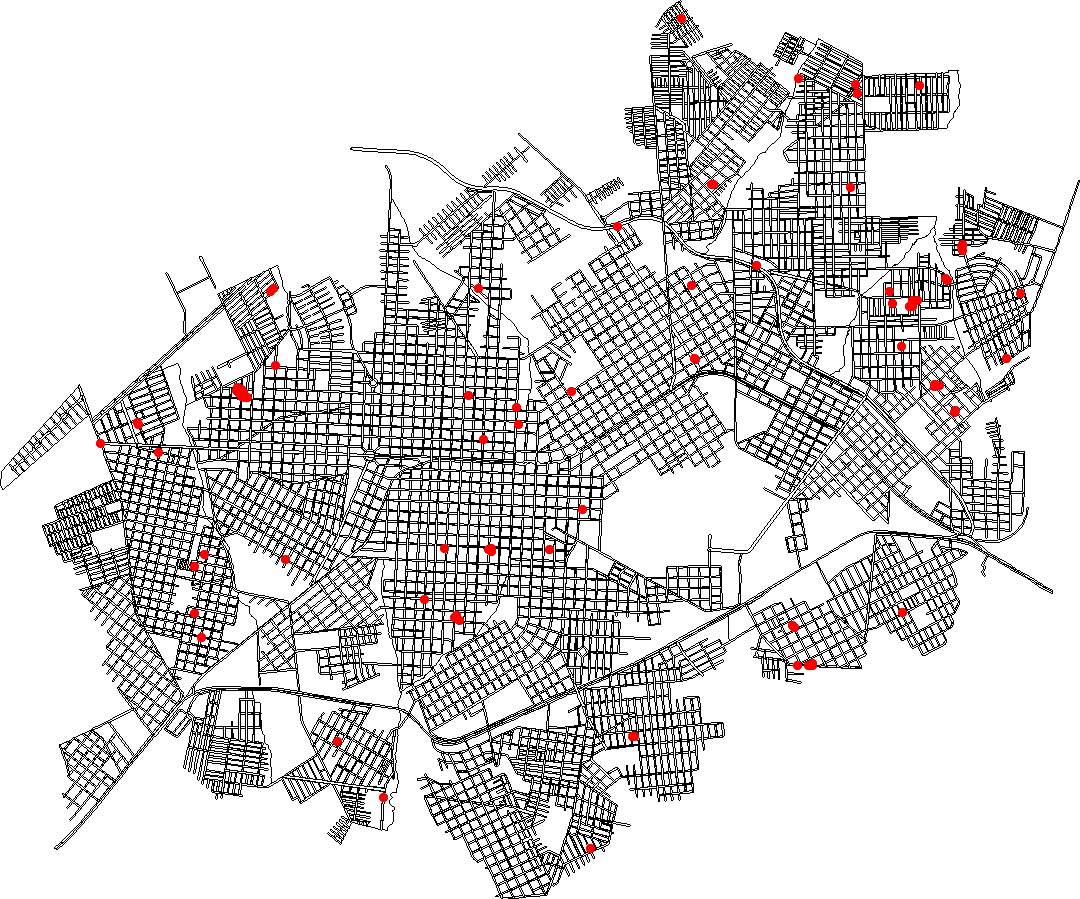
\includegraphics[width=1.0\textwidth]{Figuras/Resultados/0001/Saidas_GPU_BIT/MonteCarlo_0/Simulacao_0/Espacial/00040.png}
%     \captionsetup{labelformat=empty}
%     \captionof{figure}{Ciclo 40}
%   \end{minipage}
%   \begin{minipage}{.5\textwidth}
%     \centering
%     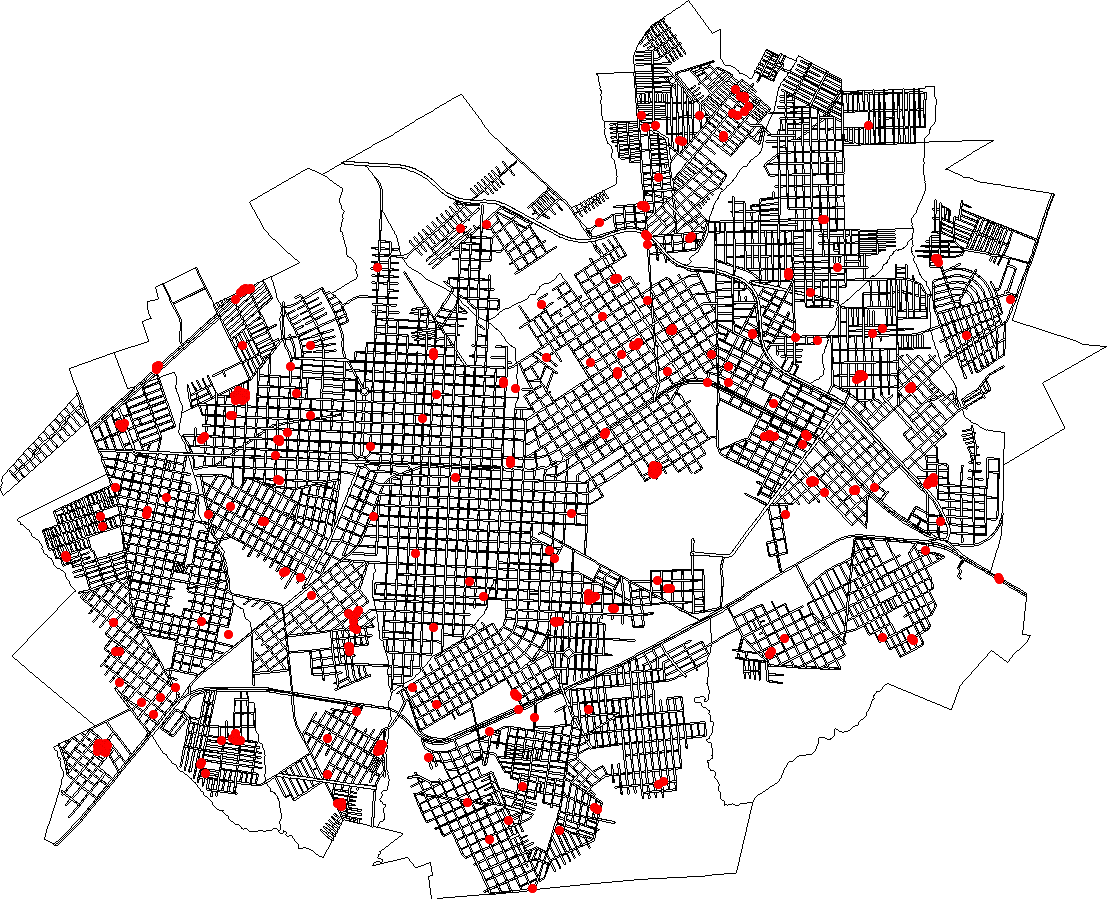
\includegraphics[width=1.0\textwidth]{Figuras/Resultados/0001/Saidas_GPU_BIT/MonteCarlo_0/Simulacao_0/Espacial/00080.png}
%     \captionsetup{labelformat=empty}
%     \captionof{figure}{Ciclo 80}
%   \end{minipage}%
%   \centering
%   \begin{minipage}{.5\textwidth}
%     \centering
%     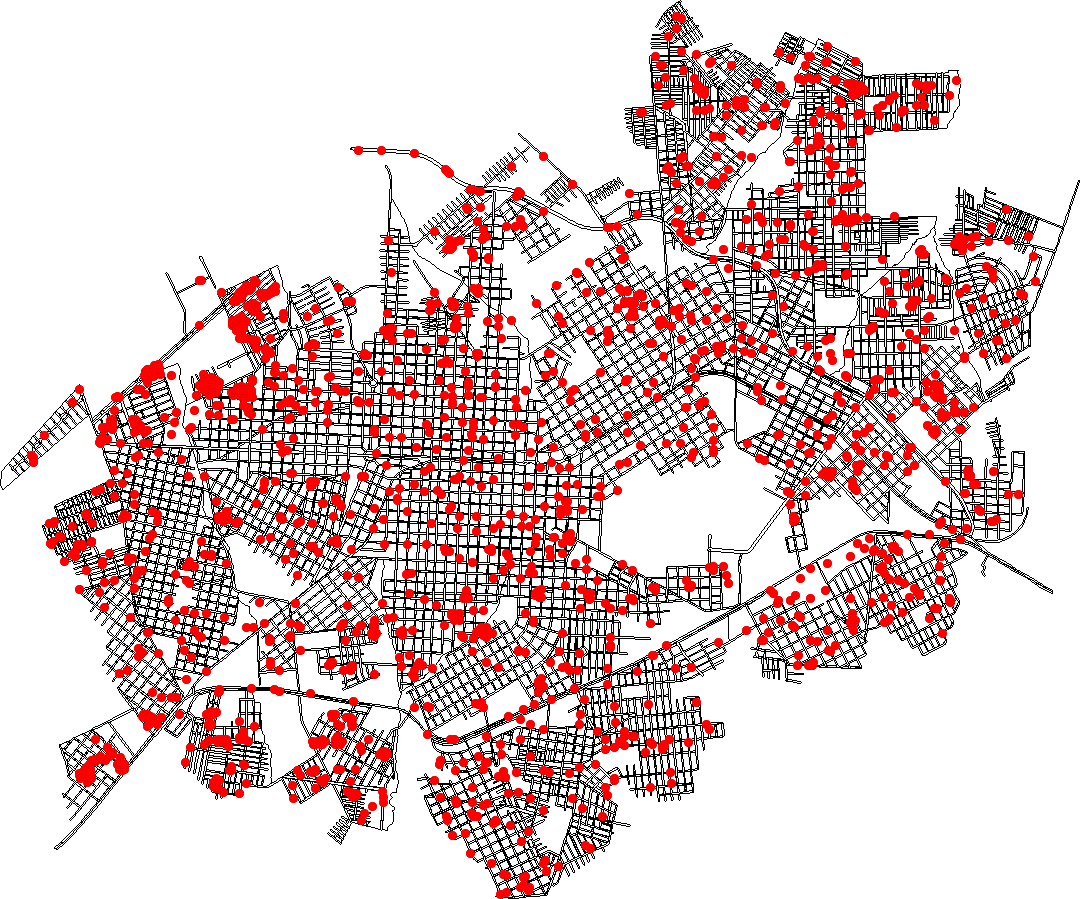
\includegraphics[width=1.0\textwidth]{Figuras/Resultados/0001/Saidas_GPU_BIT/MonteCarlo_0/Simulacao_0/Espacial/00120.png}
%     \captionsetup{labelformat=empty}
%     \captionof{figure}{Ciclo 120}
%   \end{minipage}
%   \begin{minipage}{.5\textwidth}
%     \centering
%     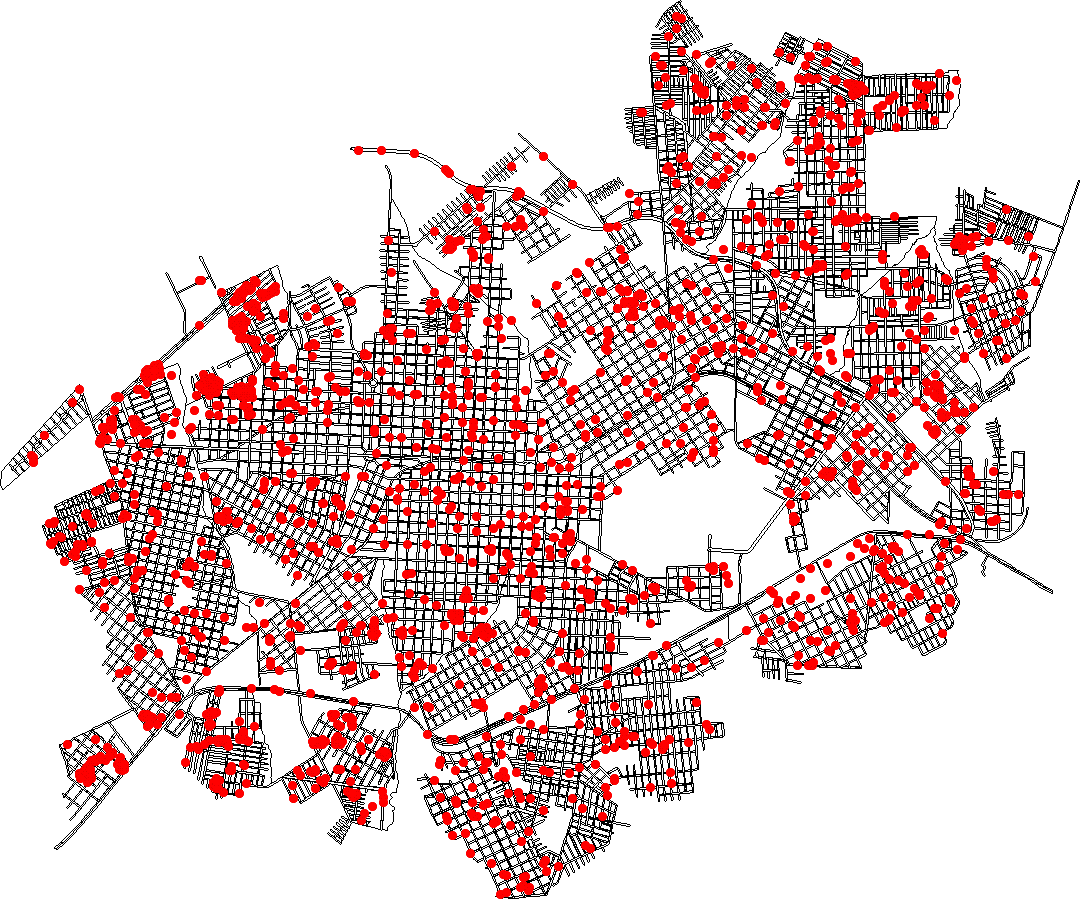
\includegraphics[width=1.0\textwidth]{Figuras/Resultados/0001/Saidas_GPU_BIT/MonteCarlo_0/Simulacao_0/Espacial/00160.png}
%     \captionsetup{labelformat=empty}
%     \captionof{figure}{Ciclo 160}
%   \end{minipage}%
%   \begin{minipage}{.5\textwidth}
%     \centering
%     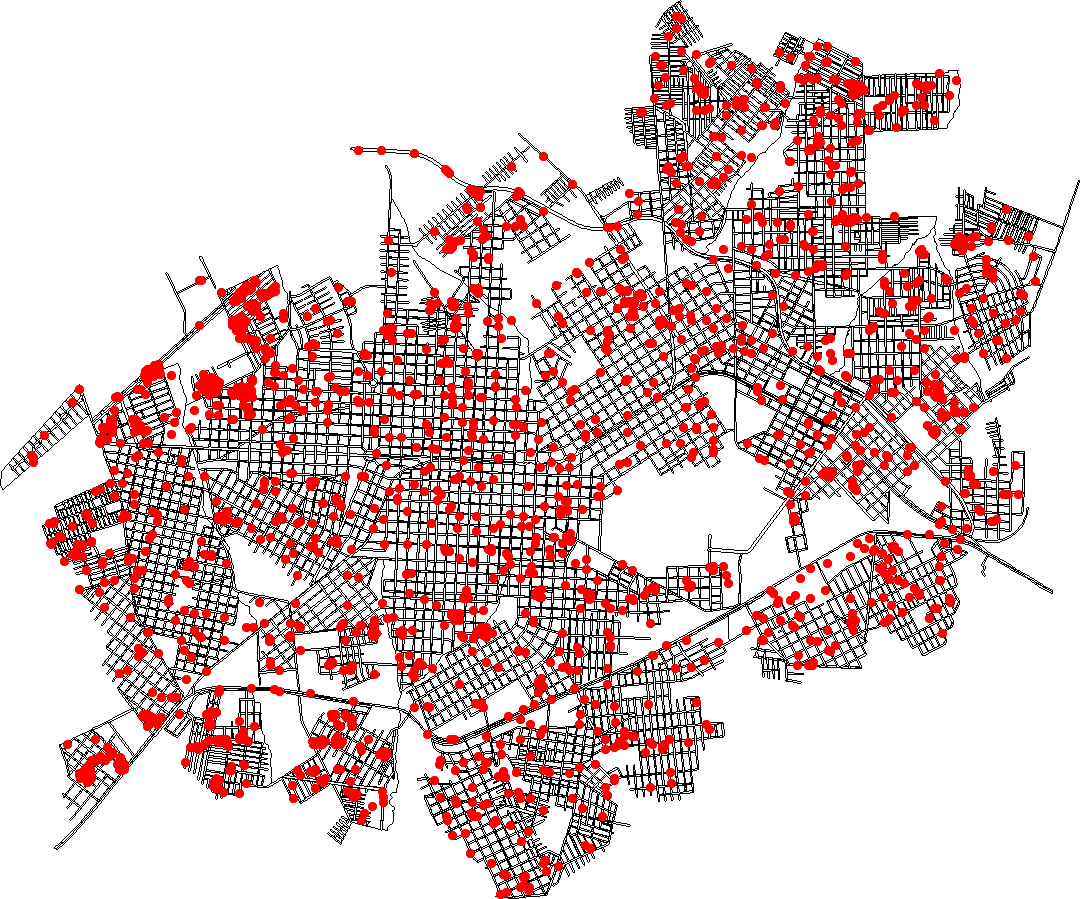
\includegraphics[width=1.0\textwidth]{Figuras/Resultados/0001/Saidas_GPU_BIT/MonteCarlo_0/Simulacao_0/Espacial/00200.png}
%     \captionsetup{labelformat=empty}
%     \captionof{figure}{Ciclo 200}
%   \end{minipage}
%   \caption{Espalhamento espacial dos agentes para o teste 0001.}
%   \label{fig:espacial_0001}
% \end{figure}
% 
% A Figura \ref{fig:espacial_observado_0001} ilustra o espalhamento espacial acumulado dos casos observados de Influenza nos meses de Julho a Dezembro de 2009.
% 
% \begin{figure}[H]
%   \centering
%   \begin{minipage}{.45\textwidth}
%     \centering
%     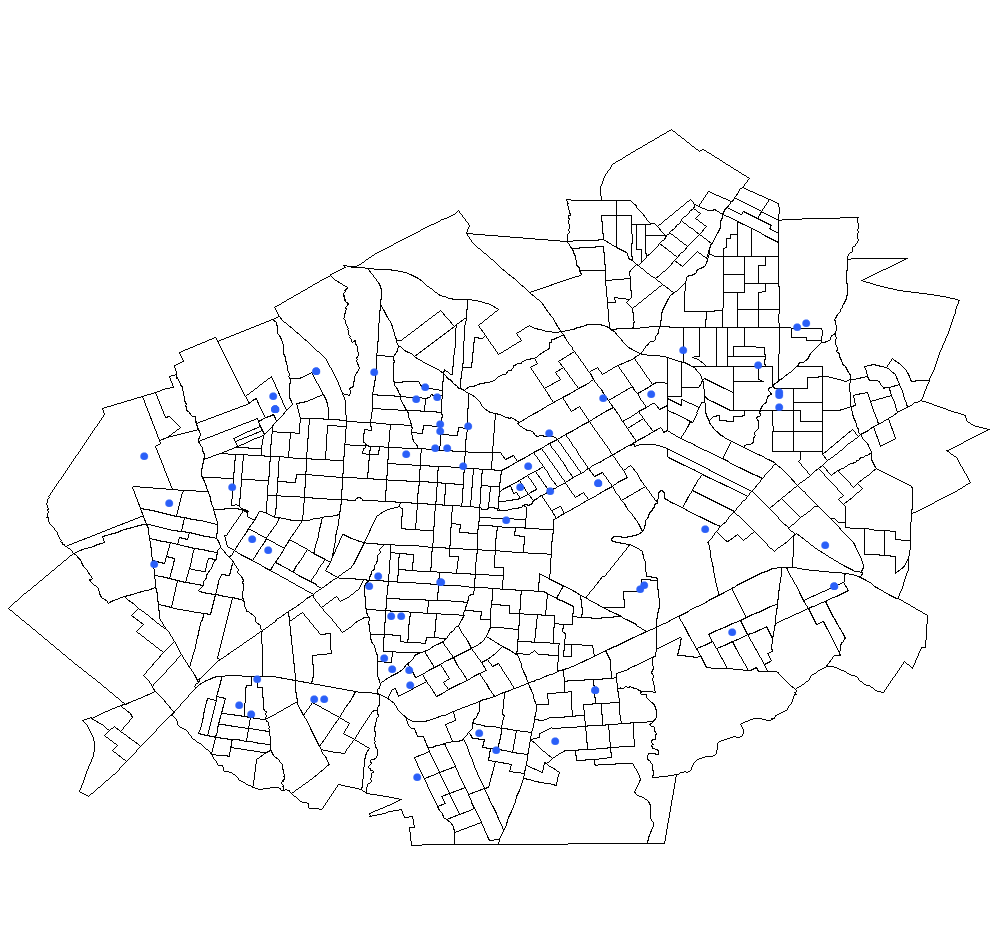
\includegraphics[width=1.0\textwidth]{Figuras/Resultados/Observado/01-07-2009.png}
%     \captionsetup{labelformat=empty}
%     \captionof{figure}{Dia 1 de Julho de 2009}
%   \end{minipage}%
%   \begin{minipage}{.45\textwidth}
%     \centering
%     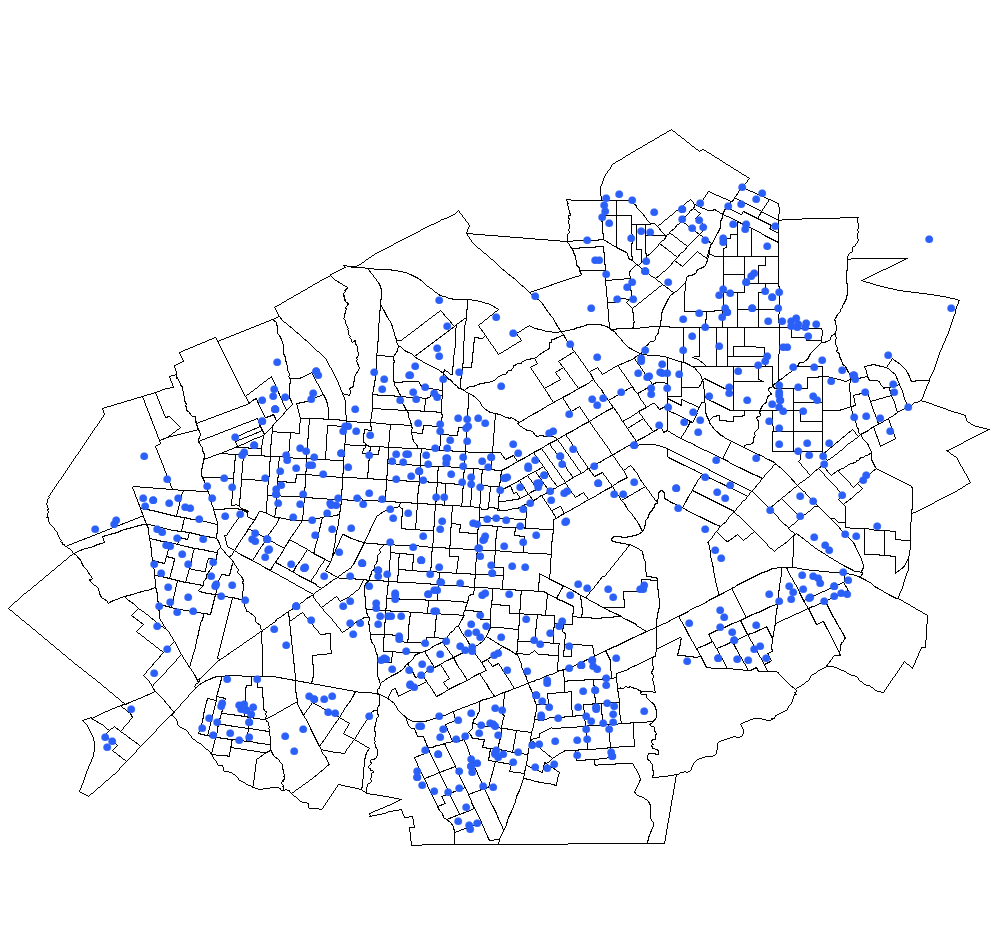
\includegraphics[width=1.0\textwidth]{Figuras/Resultados/Observado/01-08-2009.png}
%     \captionsetup{labelformat=empty}
%     \captionof{figure}{Dia 1 de Agosto de 2009}
%   \end{minipage}
%   \begin{minipage}{.45\textwidth}
%     \centering
%     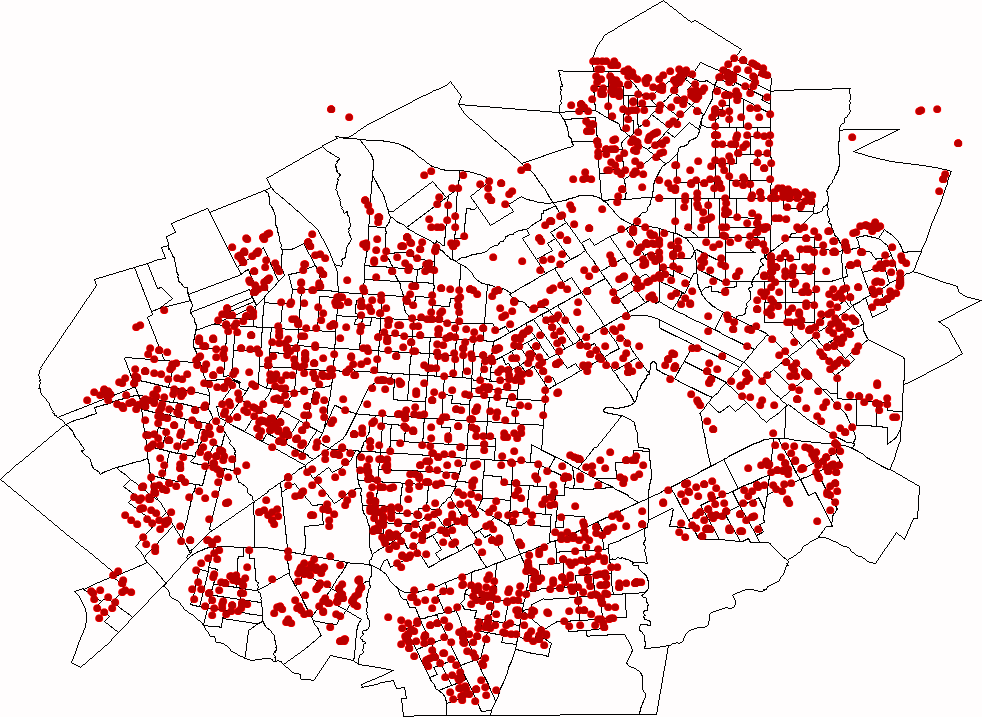
\includegraphics[width=1.0\textwidth]{Figuras/Resultados/Observado/01-09-2009.png}
%     \captionsetup{labelformat=empty}
%     \captionof{figure}{Dia 1 de Setembro de 2009}
%   \end{minipage}%
%   \centering
%   \begin{minipage}{.45\textwidth}
%     \centering
%     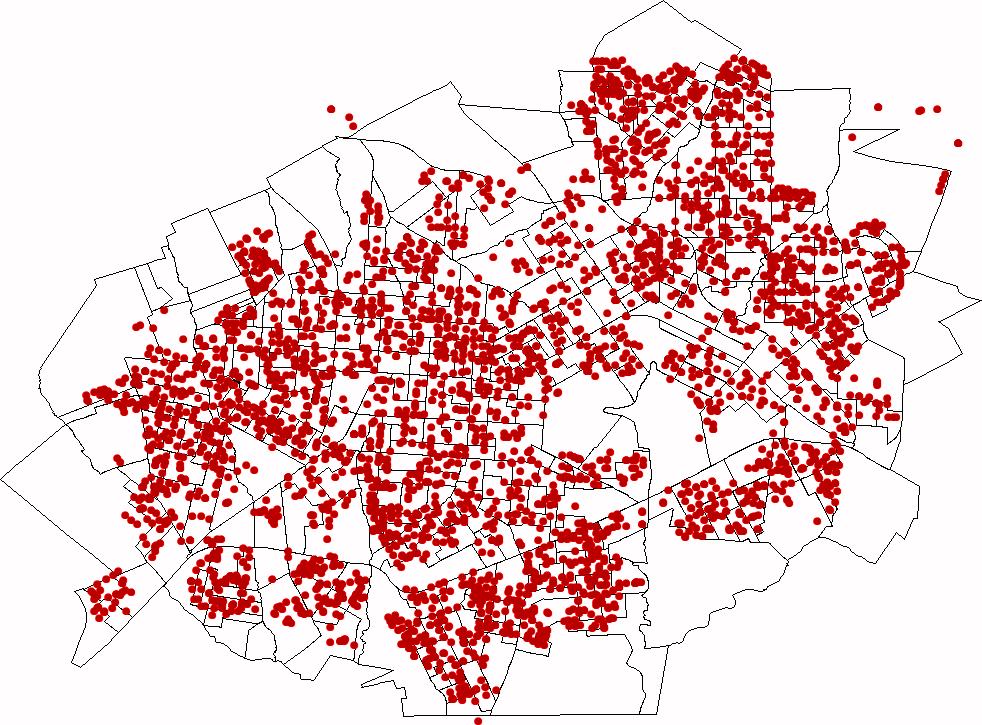
\includegraphics[width=1.0\textwidth]{Figuras/Resultados/Observado/01-10-2009.png}
%     \captionsetup{labelformat=empty}
%     \captionof{figure}{Dia 1 de Outubro de 2009}
%   \end{minipage}
%   \begin{minipage}{.45\textwidth}
%     \centering
%     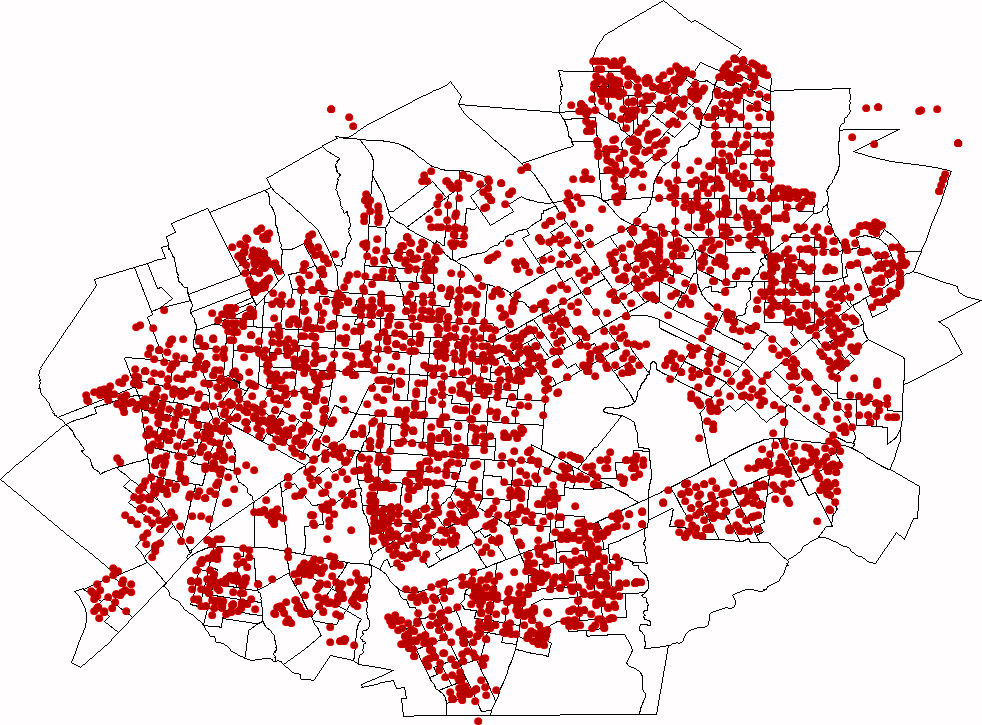
\includegraphics[width=1.0\textwidth]{Figuras/Resultados/Observado/01-11-2009.png}
%     \captionsetup{labelformat=empty}
%     \captionof{figure}{Dia 1 de Novembro de 2009}
%   \end{minipage}%
%   \begin{minipage}{.45\textwidth}
%     \centering
%     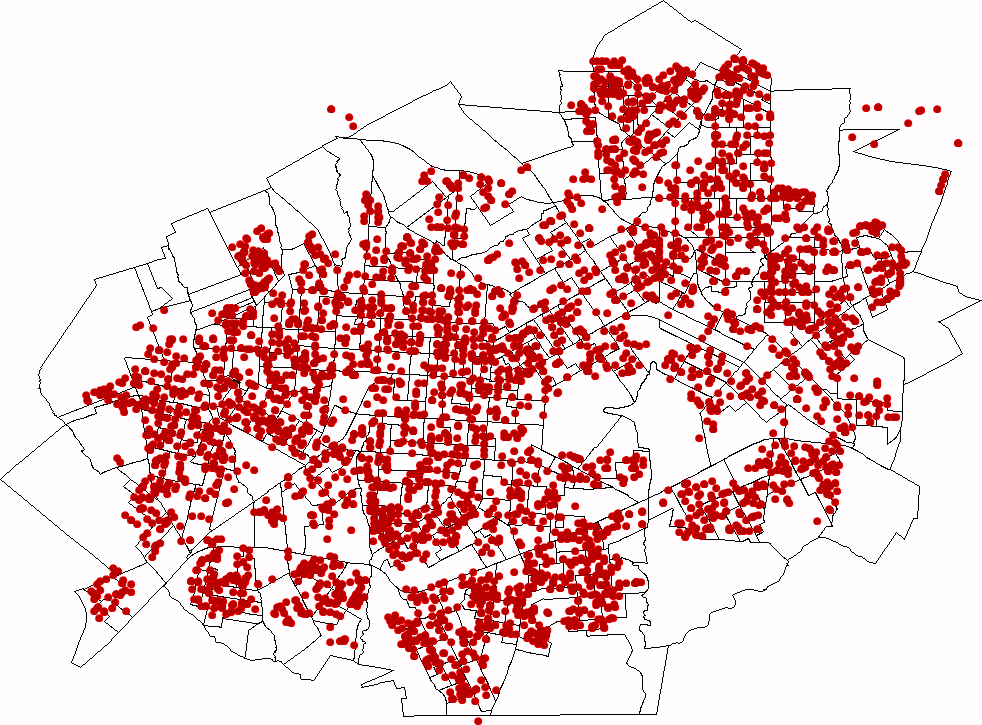
\includegraphics[width=1.0\textwidth]{Figuras/Resultados/Observado/01-12-2009.png}
%     \captionsetup{labelformat=empty}
%     \captionof{figure}{Dia 1 de Dezembro de 2009}
%   \end{minipage}
%   \caption{Espalhamento espacial observados dos casos de Influenza.}
%   \label{fig:espacial_observado_0001}
% \end{figure}
% 
% \newpage

\subsection{Teste 0002}

Em sequência são apresentados os parâmetros utilizados e resultados obtidos com a execução do teste denominado \textit{0002}. Utilizou-se o ambiente de Cascavel/PR com $286.205$ agentes. A população de agentes foi definida com base nos dados populacionais de 2010 disponibilizados pelo IBGE, que estratifica a população por faixas etárias e sexo, como ilustrado na Tabela \ref{tab:populacoes_0002}. O consumo de memória da simulação permaneceu em torno de $337,732$MB e o tempo de execução foi de $403,031$s ou $6,7171$m. \\

\begin{table}[H]
\centering
\begin{tabular}{c|c|c|c}
 \textbf{Faixa Etária} 		& \textbf{Sexo Masculino}	& \textbf{Sexo Feminino}	& \textbf{Total}	\\ \hline
  Criança			& $33.029$			& $32.029$			& $65.058$		\\
  Jovem				& $27.508$			& $27.144$			& $54.652$		\\
  Adulto			& $67.768$			& $73.023$			& $140.791$		\\
  Idoso				& $11.466$			& $14.238$ 			& $25.704$		\\ \hline
  \textbf{Total}		& $139.771$			& $146.434$			& $286.205$		\\
\end{tabular}
\caption{Tabela das populações de agentes por faixas etárias e sexos, baseada nos dados disponibilizados pelo IBGE.}
\label{tab:populacoes_0002}
\end{table}

\newpage

\textbf{Arquivo 0-SIM.csv:} 

\begin{center}
\pgfplotstabletypeset[
col sep = semicolon,
every head row/.style={before row=\toprule,after row=\midrule},
every last row/.style={after row=\bottomrule},
display columns/0/.style={string type, column type=l},
display columns/3/.style={string type, column type=l}
]{Figuras/Resultados/0002/Entradas/MonteCarlo_0/Simulacao/0-SIM.csv}
\end{center}

\textbf{Arquivo 0-INI.csv:} 

\begin{center}
\pgfplotstabletypeset[
col sep = semicolon,
every head row/.style={before row=\toprule,after row=\midrule},
every last row/.style={after row=\bottomrule},
display columns/0/.style={string type, column type=l},
display columns/3/.style={string type, column type=l}
]{Figuras/Resultados/0002/Entradas/MonteCarlo_0/Humanos/0-INI.csv}
\end{center}

\textbf{Arquivo 1-MOV.csv:} 

\begin{center}
\pgfplotstabletypeset[
col sep = semicolon,
every head row/.style={before row=\toprule,after row=\midrule},
every last row/.style={after row=\bottomrule},
display columns/0/.style={string type, column type=l},
display columns/3/.style={string type, column type=l}
]{Figuras/Resultados/0002/Entradas/MonteCarlo_0/Humanos/1-MOV.csv}
\end{center}

\textbf{Arquivo 2-CON.csv:} 

\begin{center}
\pgfplotstabletypeset[
col sep = semicolon,
every head row/.style={before row=\toprule,after row=\midrule},
every last row/.style={after row=\bottomrule},
display columns/0/.style={string type, column type=l},
display columns/3/.style={string type, column type=l}
]{Figuras/Resultados/0002/Entradas/MonteCarlo_0/Humanos/2-CON.csv}
\end{center}

\textbf{Arquivo 3-TRA.csv:} 

\begin{center}
\pgfplotstabletypeset[
col sep = semicolon,
every head row/.style={before row=\toprule,after row=\midrule},
every last row/.style={after row=\bottomrule},
display columns/0/.style={string type, column type=l},
display columns/3/.style={string type, column type=l}
]{Figuras/Resultados/0002/Entradas/MonteCarlo_0/Humanos/3-TRA.csv}
\end{center}

\newpage

\subsubsection{Quantidades de Agentes Infectados Acumulados ao Longo do Tempo de Simulação}

A Figura \ref{fig:Quantidades_Agentes_Infectados_Acumulado_0002} ilustra as quantidades de agentes infectados acumulados.

\begin{figure}[H]
  \centering
  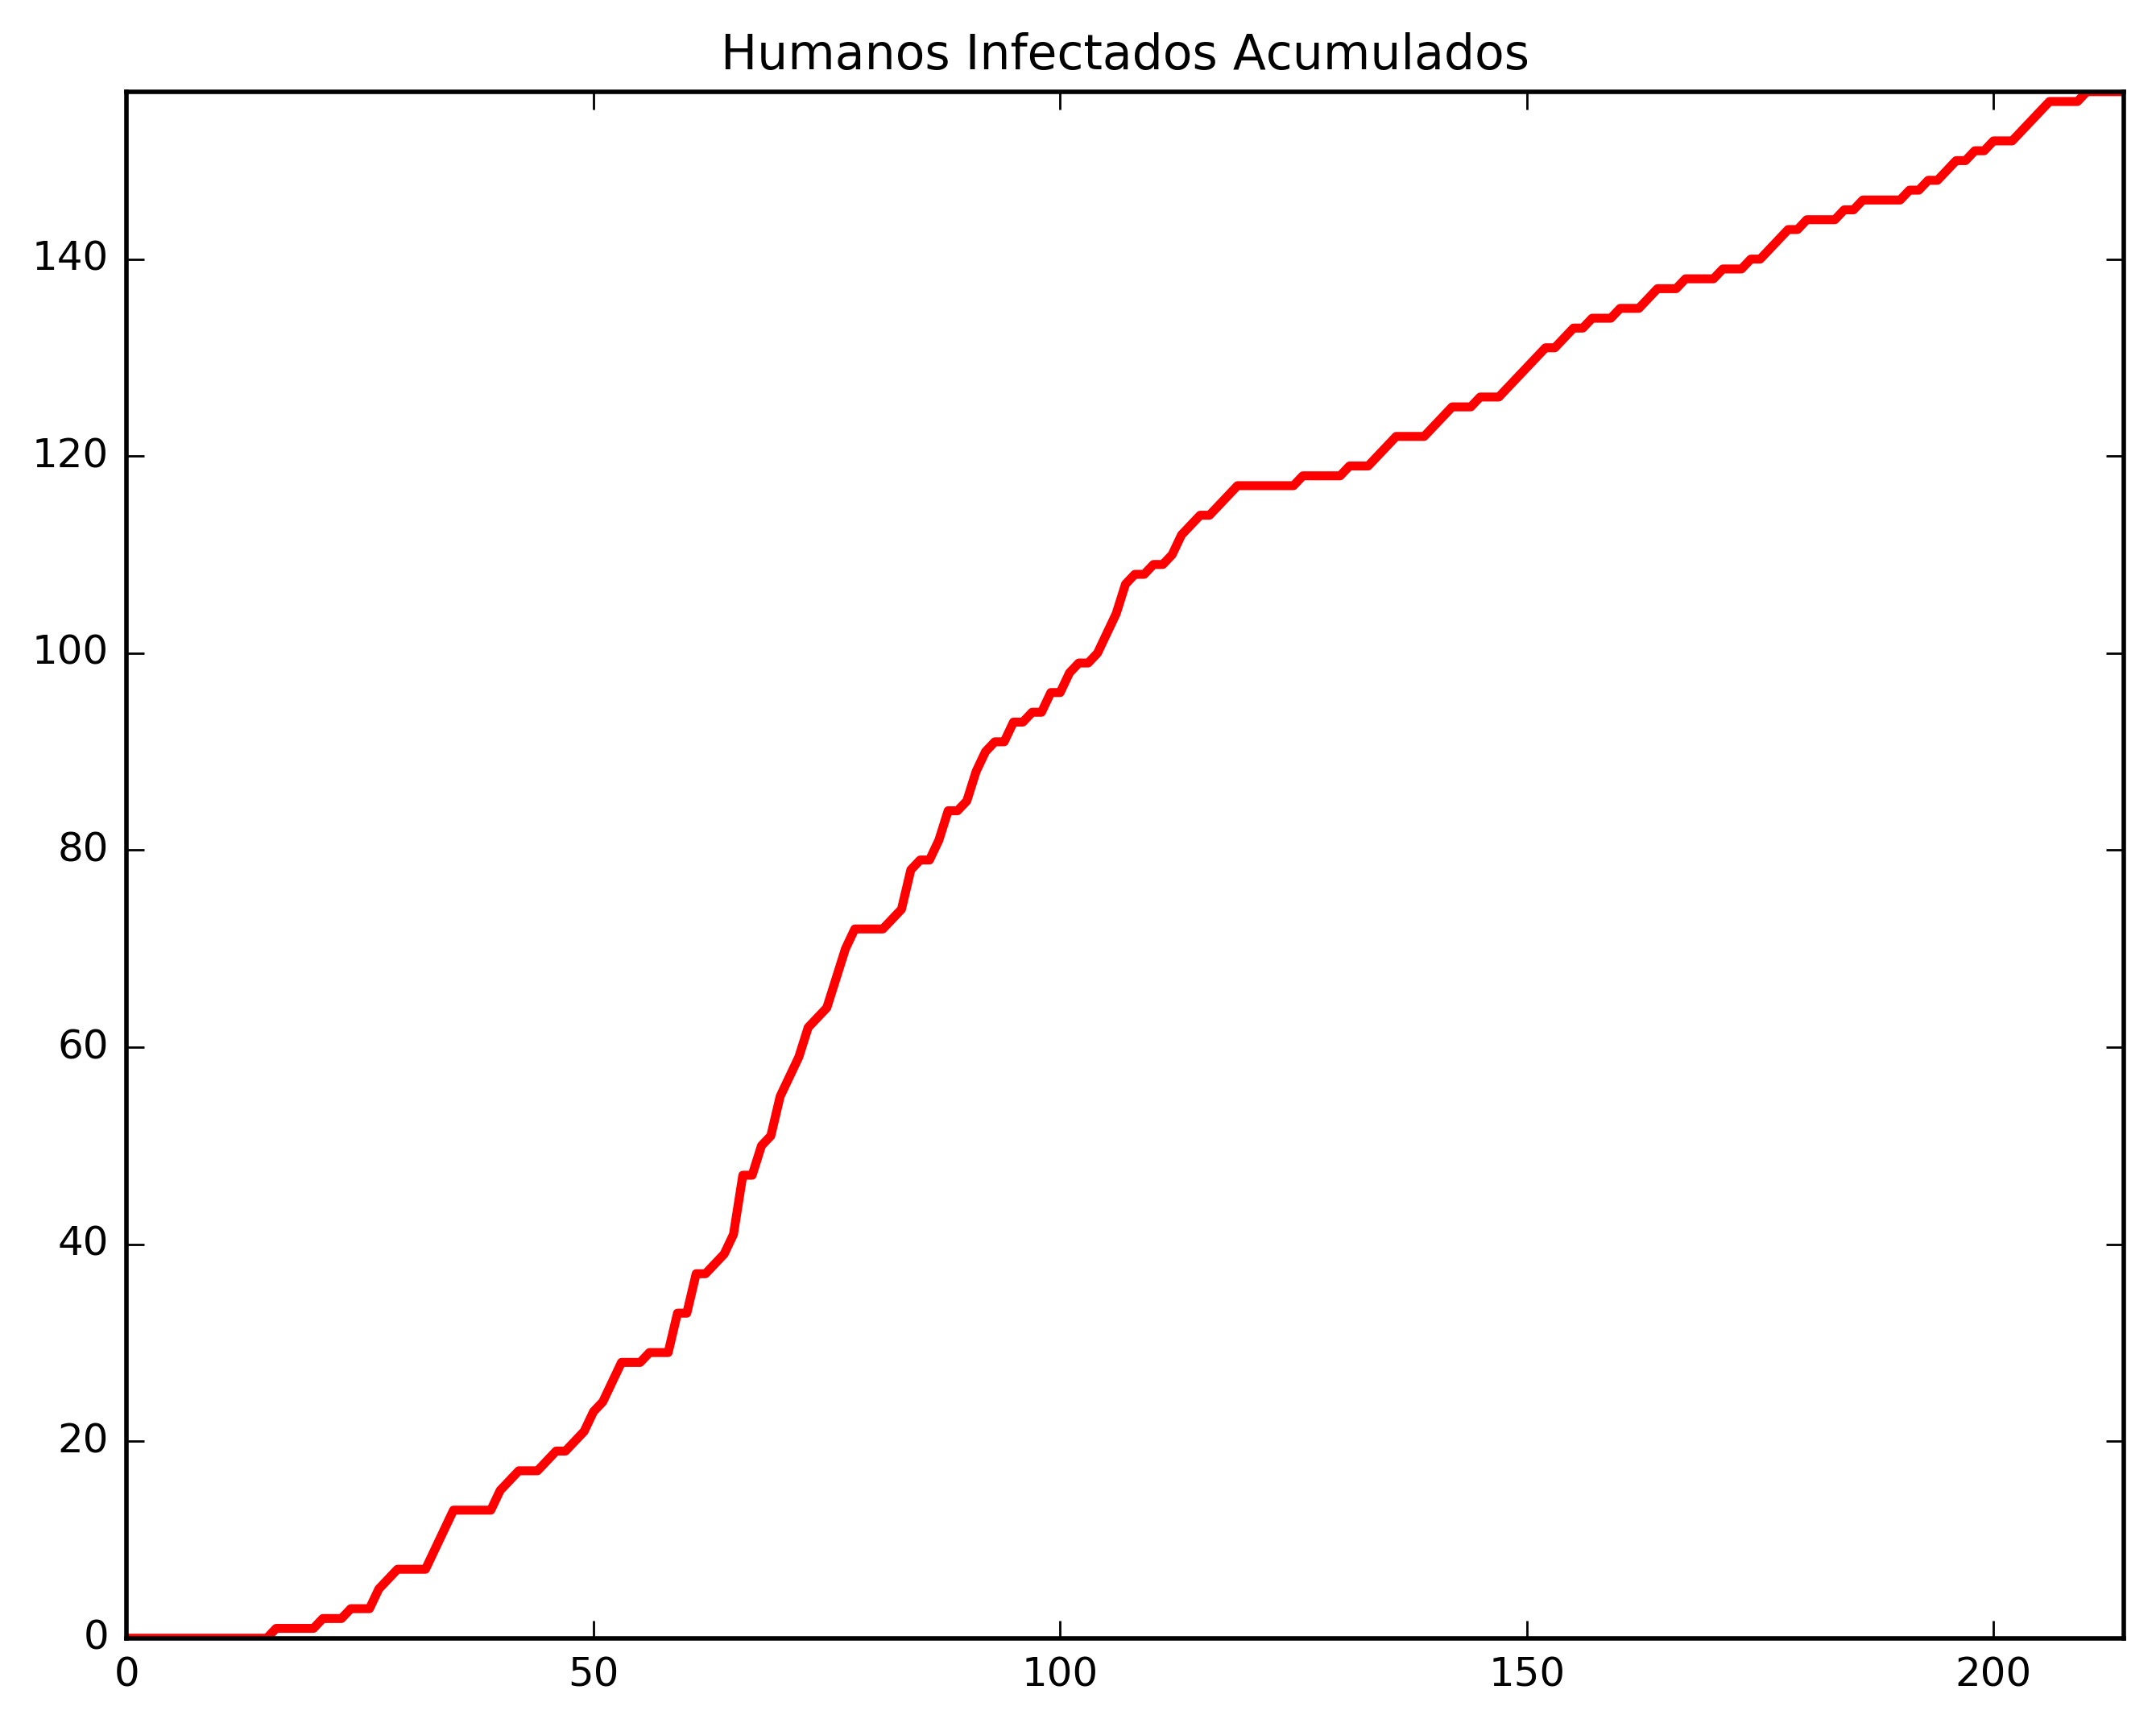
\includegraphics[width=1.0\textwidth]{Figuras/Resultados/0002/Saidas/MonteCarlo_0/Quantidades_Humanos_Novo_Total.png}
  \caption{Quantidades de agentes infectados acumulados.}
  \label{fig:Quantidades_Agentes_Infectados_Acumulado_0002}
\end{figure}

A Figura \ref{fig:Casos_Observados_Acumulados_0002} ilustra as quantidades de casos observados acumulados.

\begin{figure}[H]
  \centering
  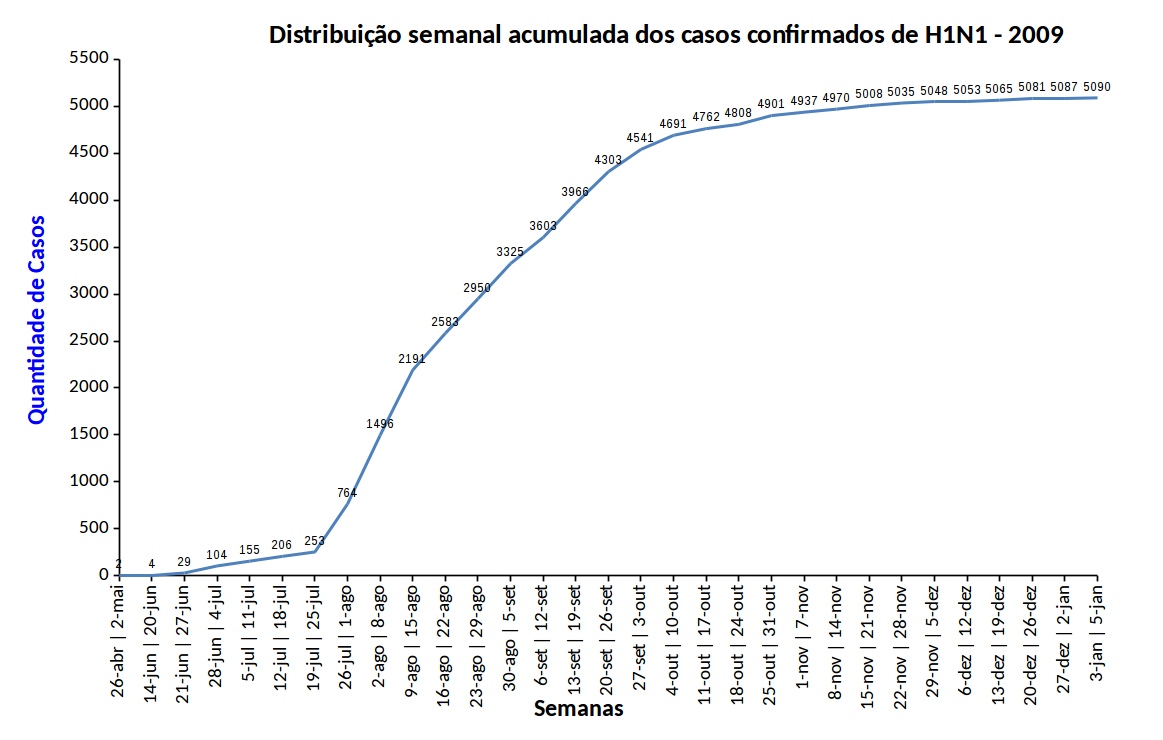
\includegraphics[width=1.0\textwidth]{Figuras/Resultados/Observado/Casos_Observados_Acumulados.png}
  \caption{Quantidades de casos observados acumulados.}
  \label{fig:Casos_Observados_Acumulados_0002}
\end{figure}

\newpage

\subsubsection{Espalhamento Espacial dos Agentes Humanos ao Longo do Tempo de Simulação}

A Figura \ref{fig:casos_0002} ilustra o espalhamento espacial dos agentes humanos no ambiente nos ciclos 1, 40, 80, 120, 160 e 200.

\begin{figure}[H]
  \centering
  \begin{minipage}{.5\textwidth}
    \centering
    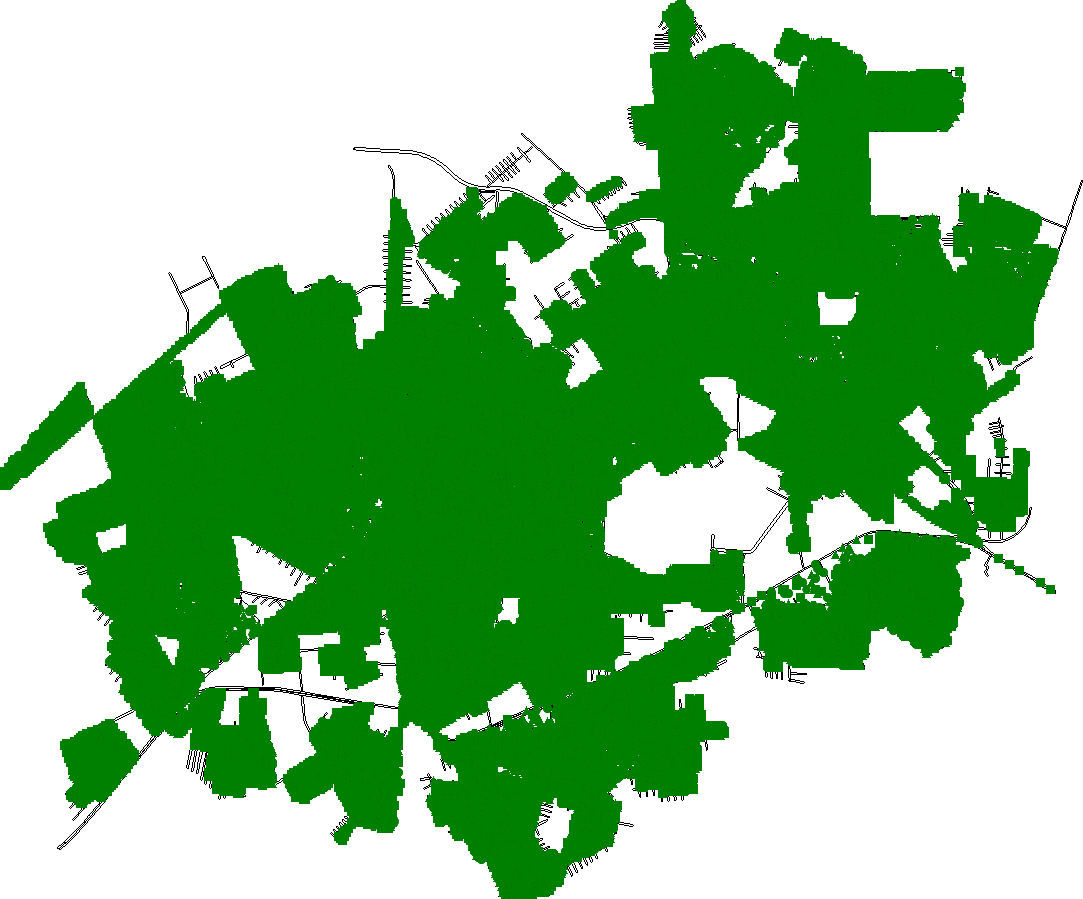
\includegraphics[width=1.0\textwidth]{Figuras/Resultados/0002/Saidas/MonteCarlo_0/Simulacao_0/Espacial/00000.png}
    \captionsetup{labelformat=empty}
    \captionof{figure}{Ciclo 1}
  \end{minipage}%
  \begin{minipage}{.5\textwidth}
    \centering
    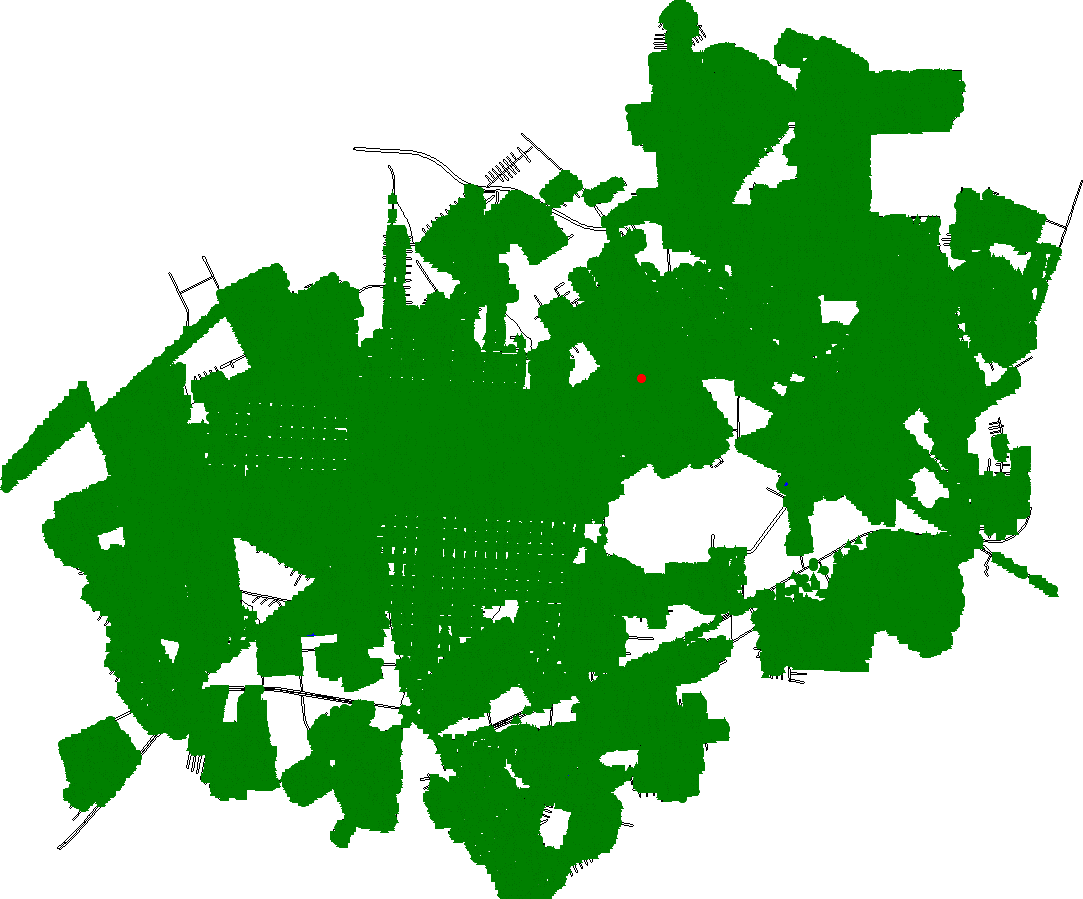
\includegraphics[width=1.0\textwidth]{Figuras/Resultados/0002/Saidas/MonteCarlo_0/Simulacao_0/Espacial/00004.png}
    \captionsetup{labelformat=empty}
    \captionof{figure}{Ciclo 40}
  \end{minipage}
  \begin{minipage}{.5\textwidth}
    \centering
    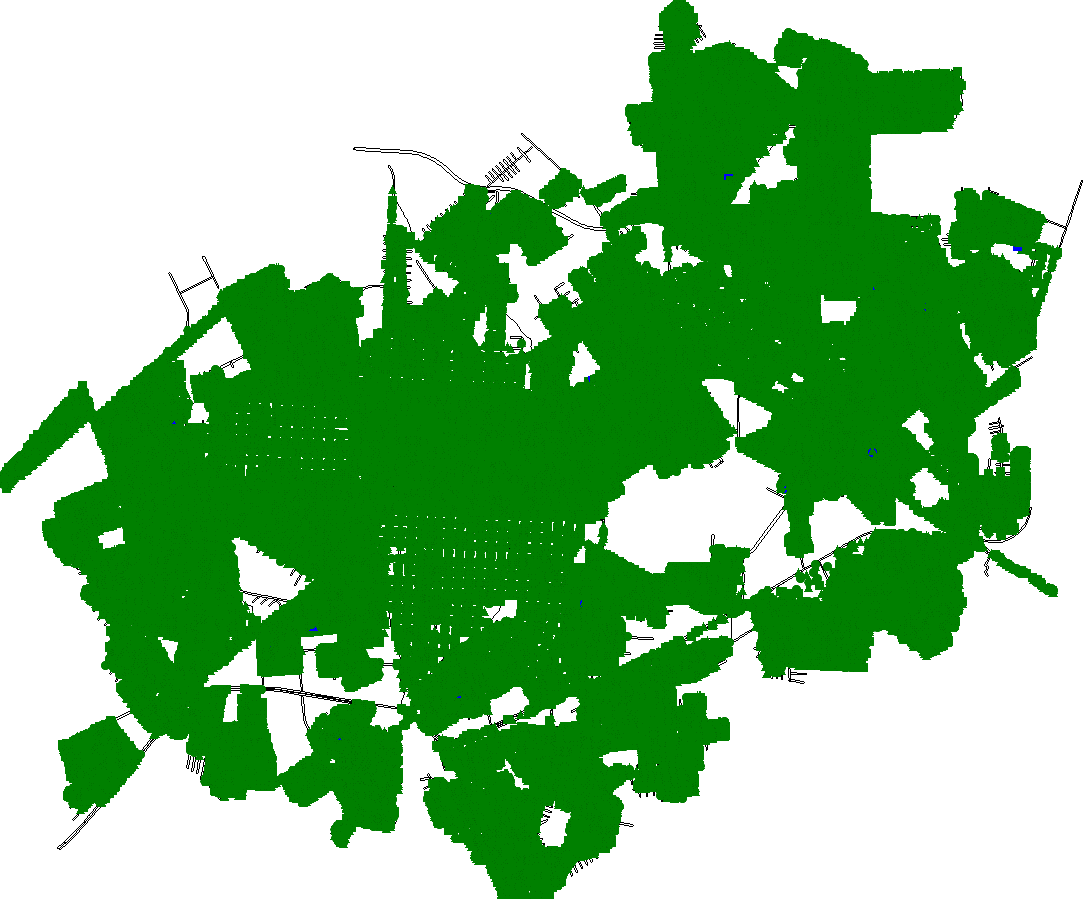
\includegraphics[width=1.0\textwidth]{Figuras/Resultados/0002/Saidas/MonteCarlo_0/Simulacao_0/Espacial/00008.png}
    \captionsetup{labelformat=empty}
    \captionof{figure}{Ciclo 80}
  \end{minipage}%
  \centering
  \begin{minipage}{.5\textwidth}
    \centering
    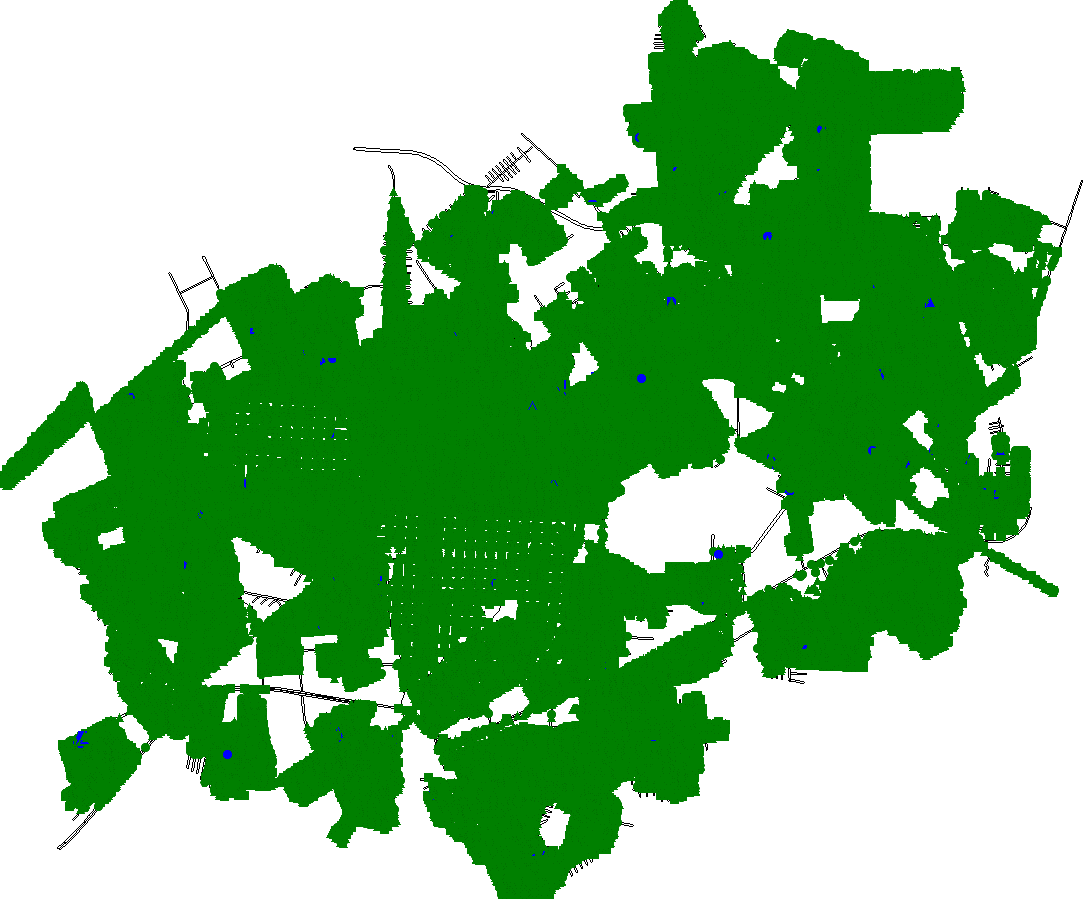
\includegraphics[width=1.0\textwidth]{Figuras/Resultados/0002/Saidas/MonteCarlo_0/Simulacao_0/Espacial/00012.png}
    \captionsetup{labelformat=empty}
    \captionof{figure}{Ciclo 120}
  \end{minipage}
  \begin{minipage}{.5\textwidth}
    \centering
    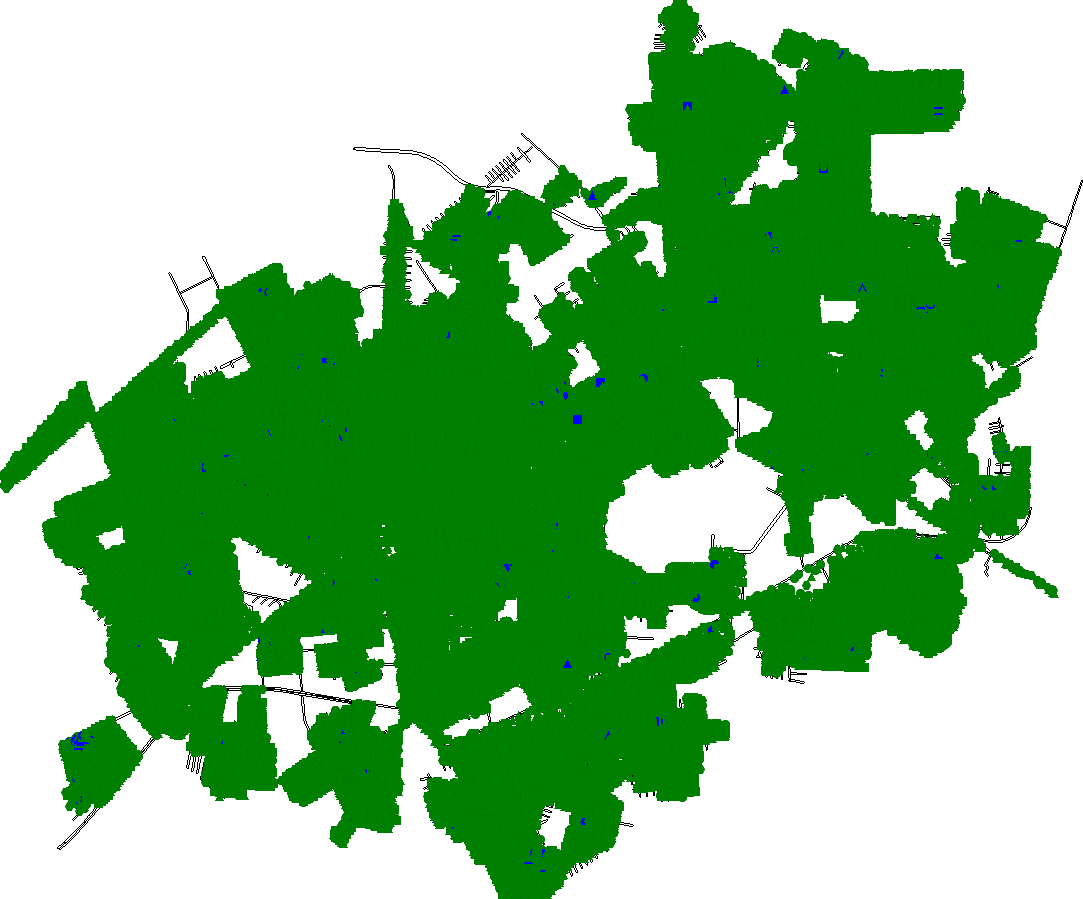
\includegraphics[width=1.0\textwidth]{Figuras/Resultados/0002/Saidas/MonteCarlo_0/Simulacao_0/Espacial/00016.png}
    \captionsetup{labelformat=empty}
    \captionof{figure}{Ciclo 160}
  \end{minipage}%
  \begin{minipage}{.5\textwidth}
    \centering
    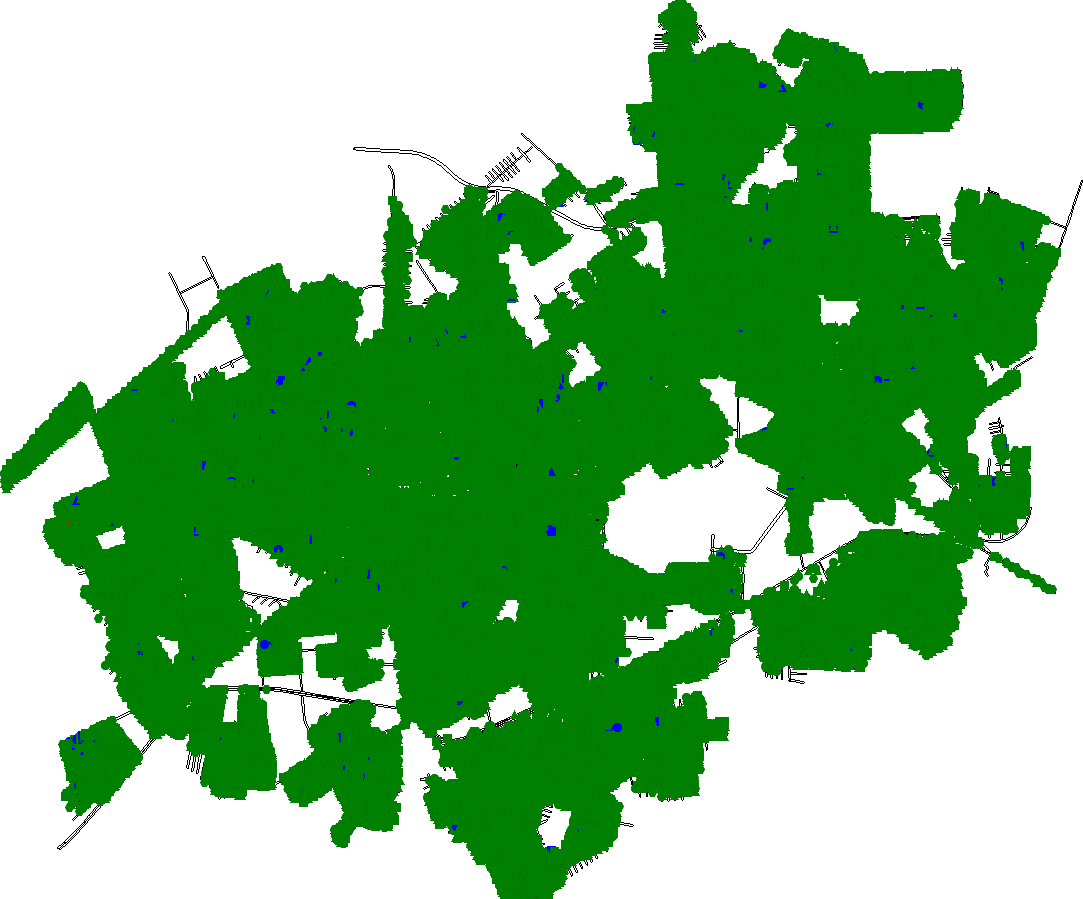
\includegraphics[width=1.0\textwidth]{Figuras/Resultados/0002/Saidas/MonteCarlo_0/Simulacao_0/Espacial/00020.png}
    \captionsetup{labelformat=empty}
    \captionof{figure}{Ciclo 200}
  \end{minipage}
  \caption{Espalhamento espacial dos agentes humanos no ambiente para o teste 0002.}
  \label{fig:casos_0002}
\end{figure}

\subsubsection{Espalhamento Espacial Acumulado dos Agentes Infectados ao Longo do Tempo de Simulação}

A Figura \ref{fig:espacial_0002} ilustra o espalhamento espacial acumulado dos agentes infectados no ambiente nos ciclos 1, 40, 80, 120, 160 e 200.

\begin{figure}[H]
  \centering
  \begin{minipage}{.5\textwidth}
    \centering
    \includegraphics[width=1.0\textwidth]{Figuras/Resultados/0002/Saidas/MonteCarlo_0/Simulacao_0/Acumulado/00000.png}
    \captionsetup{labelformat=empty}
    \captionof{figure}{Ciclo 1}
  \end{minipage}%
  \begin{minipage}{.5\textwidth}
    \centering
    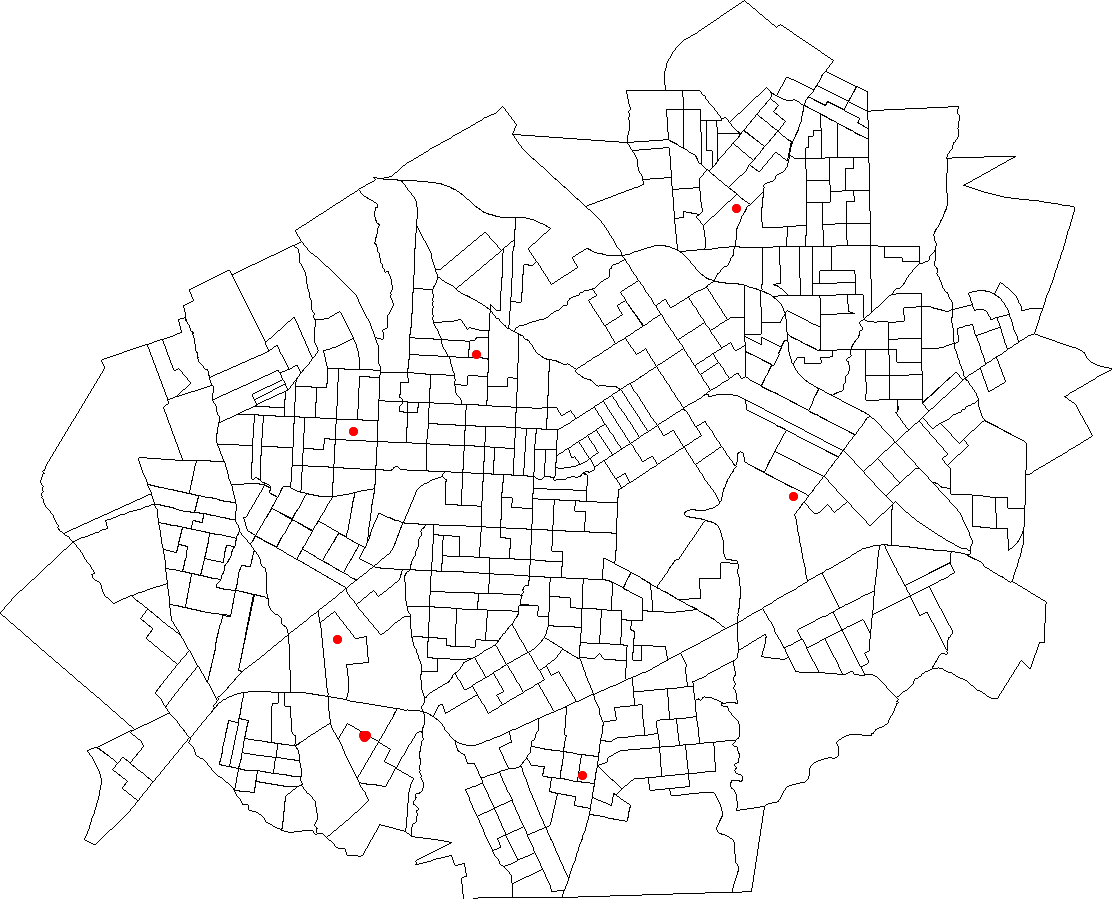
\includegraphics[width=1.0\textwidth]{Figuras/Resultados/0002/Saidas/MonteCarlo_0/Simulacao_0/Acumulado/00004.png}
    \captionsetup{labelformat=empty}
    \captionof{figure}{Ciclo 40}
  \end{minipage}
  \begin{minipage}{.5\textwidth}
    \centering
    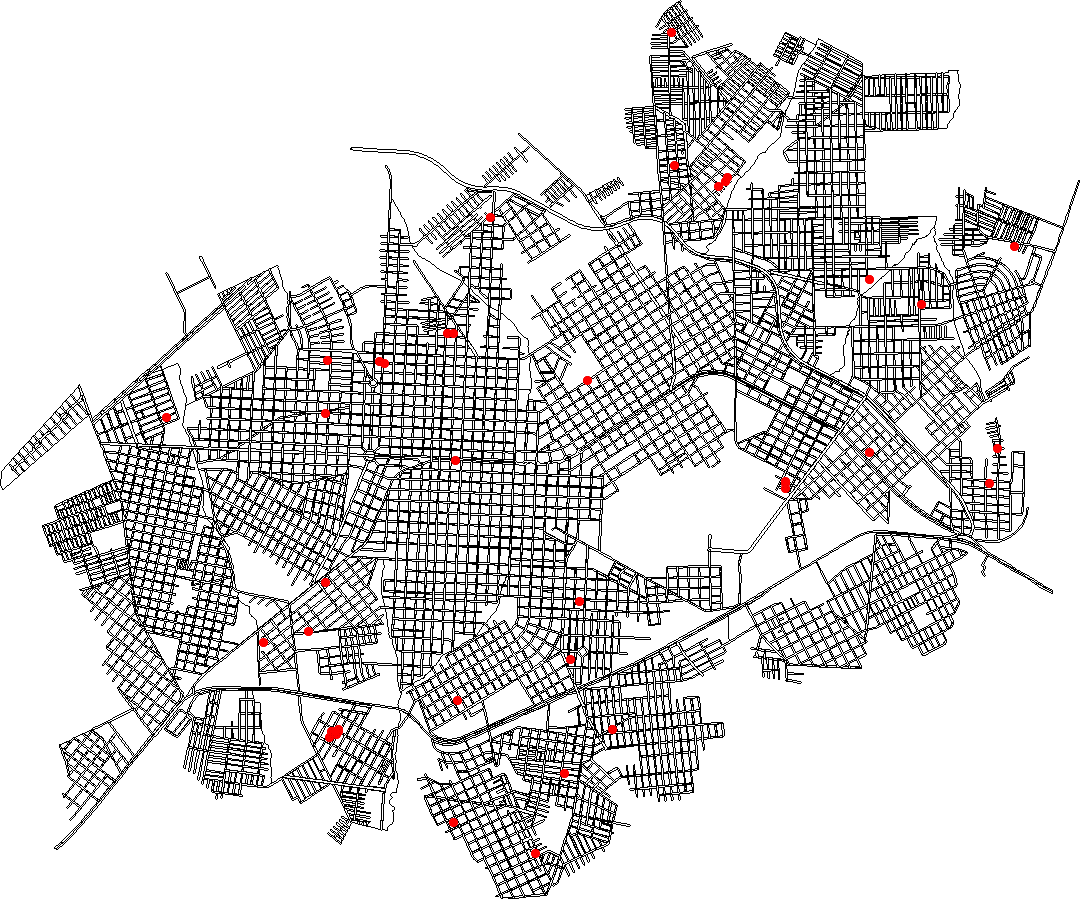
\includegraphics[width=1.0\textwidth]{Figuras/Resultados/0002/Saidas/MonteCarlo_0/Simulacao_0/Acumulado/00008.png}
    \captionsetup{labelformat=empty}
    \captionof{figure}{Ciclo 80}
  \end{minipage}%
  \centering
  \begin{minipage}{.5\textwidth}
    \centering
    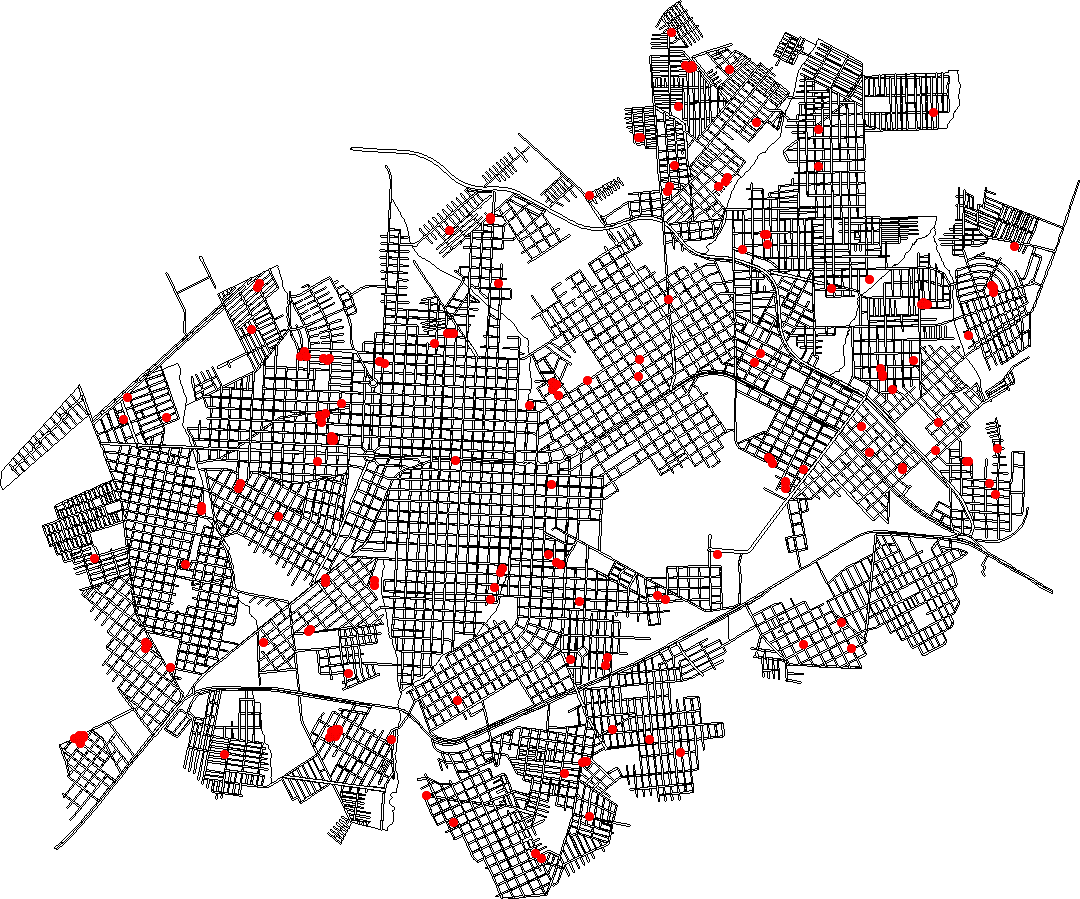
\includegraphics[width=1.0\textwidth]{Figuras/Resultados/0002/Saidas/MonteCarlo_0/Simulacao_0/Acumulado/00012.png}
    \captionsetup{labelformat=empty}
    \captionof{figure}{Ciclo 120}
  \end{minipage}
  \begin{minipage}{.5\textwidth}
    \centering
    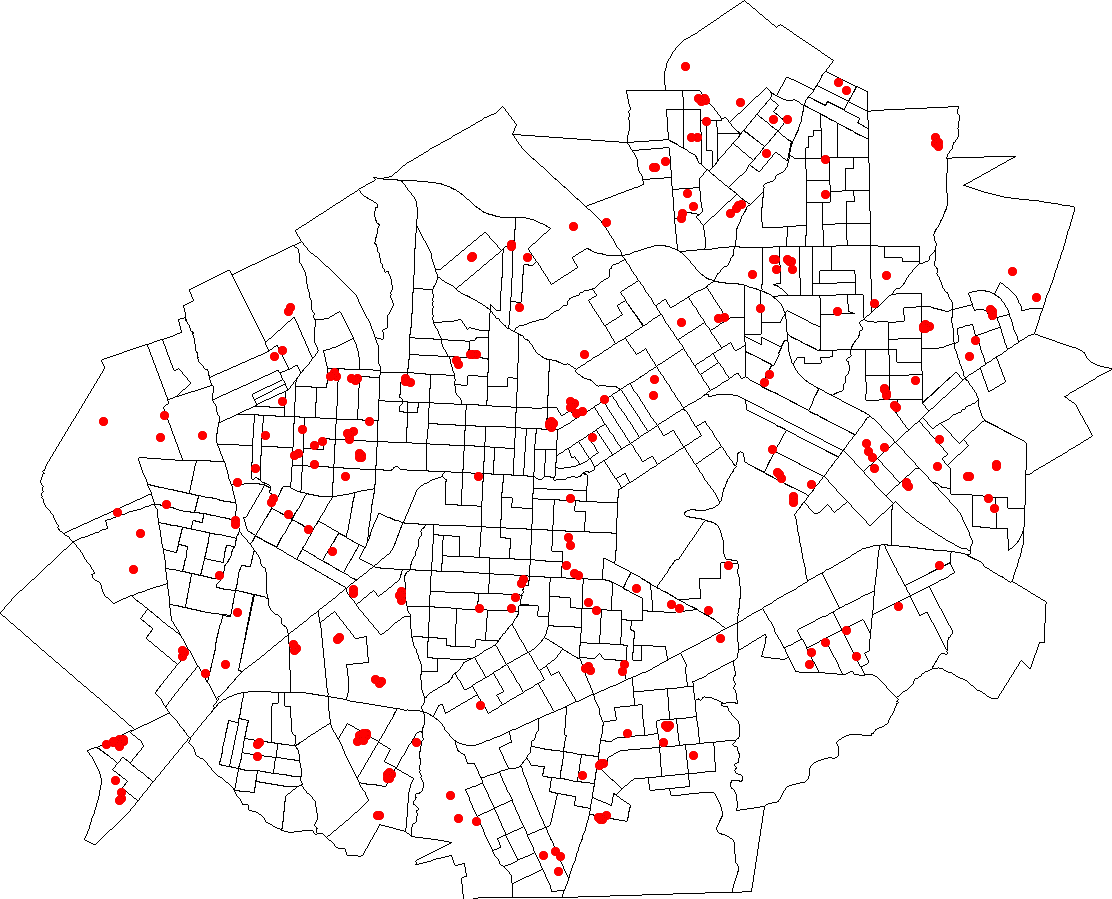
\includegraphics[width=1.0\textwidth]{Figuras/Resultados/0002/Saidas/MonteCarlo_0/Simulacao_0/Acumulado/00016.png}
    \captionsetup{labelformat=empty}
    \captionof{figure}{Ciclo 160}
  \end{minipage}%
  \begin{minipage}{.5\textwidth}
    \centering
    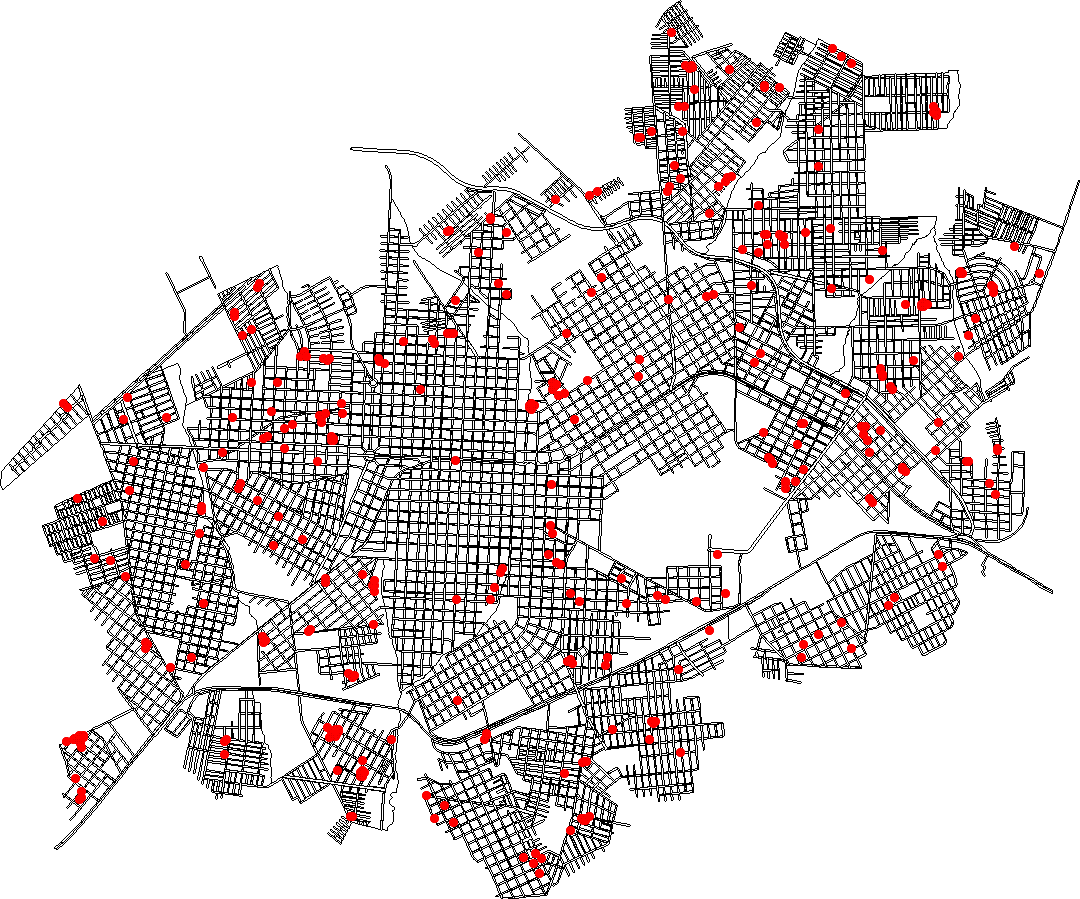
\includegraphics[width=1.0\textwidth]{Figuras/Resultados/0002/Saidas/MonteCarlo_0/Simulacao_0/Acumulado/00020.png}
    \captionsetup{labelformat=empty}
    \captionof{figure}{Ciclo 200}
  \end{minipage}
  \caption{Espalhamento espacial dos agentes para o teste 0002.}
  \label{fig:espacial_0002}
\end{figure}

A Figura \ref{fig:espacial_observado_0002} ilustra o espalhamento espacial acumulado dos casos observados de Influenza nos meses de Julho a Dezembro de 2009.

\begin{figure}[H]
  \centering
  \begin{minipage}{.45\textwidth}
    \centering
    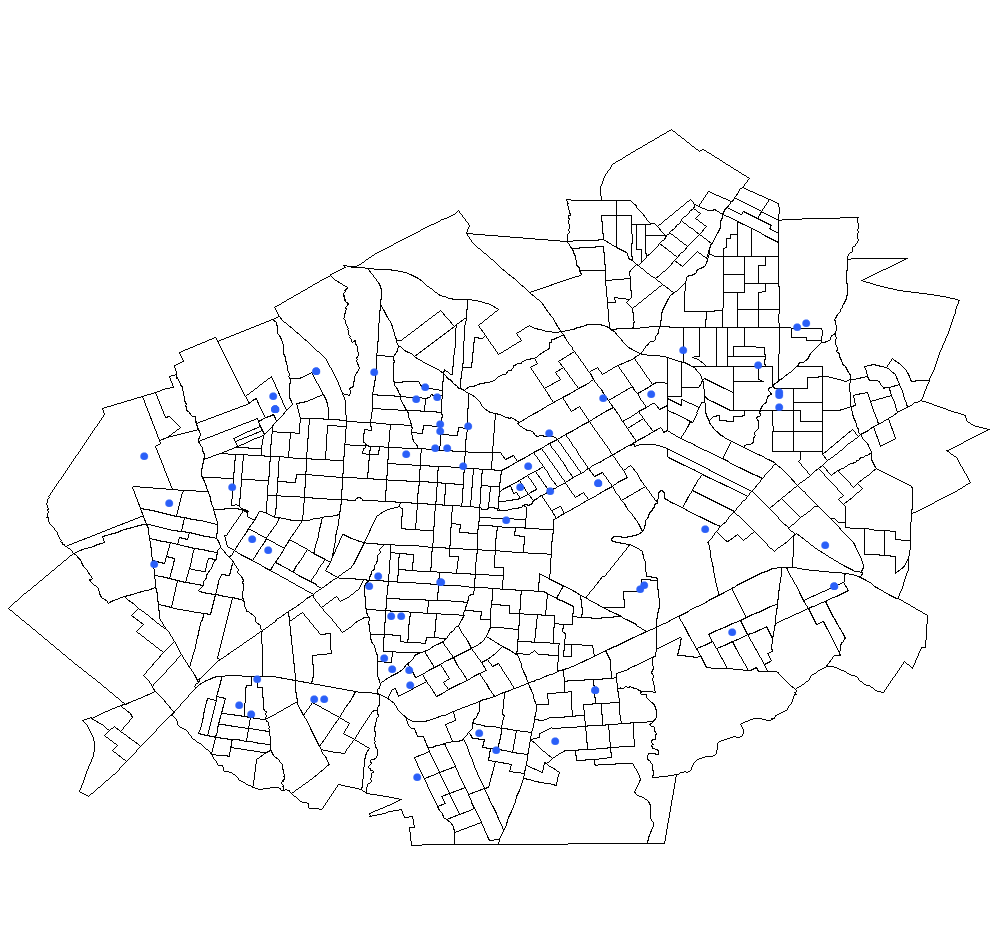
\includegraphics[width=1.0\textwidth]{Figuras/Resultados/Observado/01-07-2009.png}
    \captionsetup{labelformat=empty}
    \captionof{figure}{Dia 1 de Julho de 2009}
  \end{minipage}%
  \begin{minipage}{.45\textwidth}
    \centering
    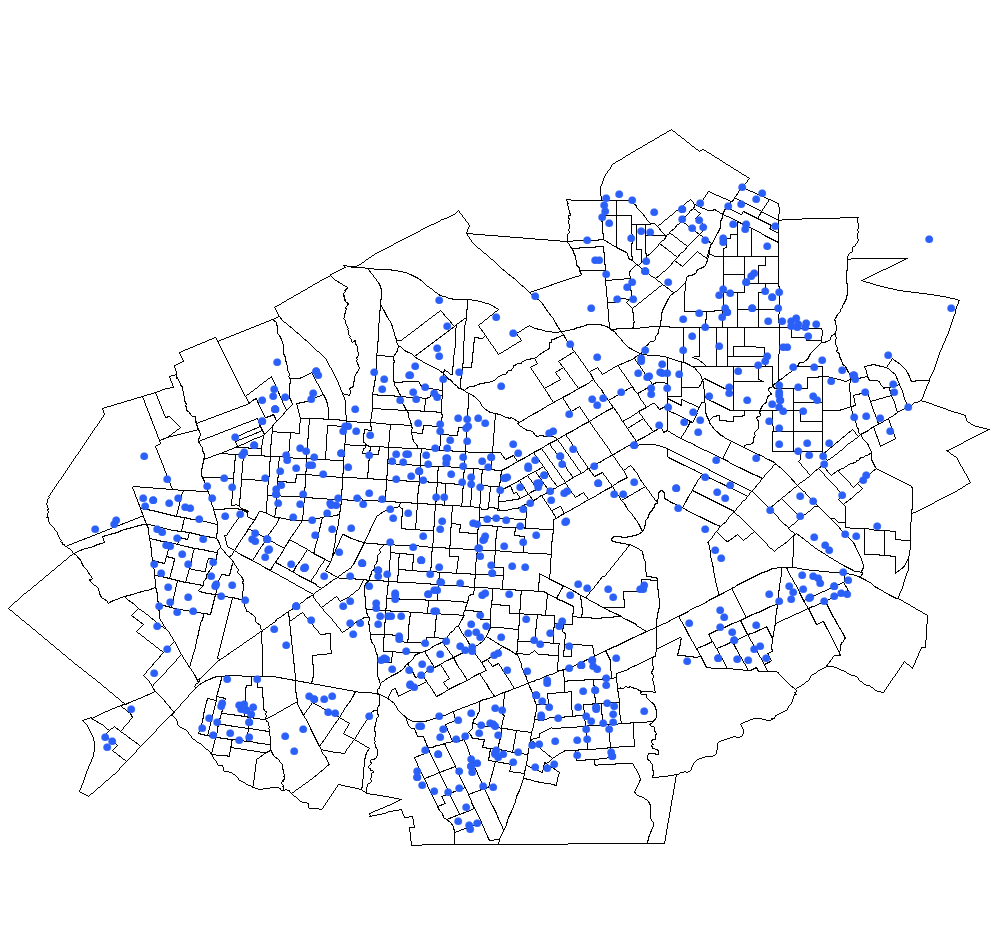
\includegraphics[width=1.0\textwidth]{Figuras/Resultados/Observado/01-08-2009.png}
    \captionsetup{labelformat=empty}
    \captionof{figure}{Dia 1 de Agosto de 2009}
  \end{minipage}
  \begin{minipage}{.45\textwidth}
    \centering
    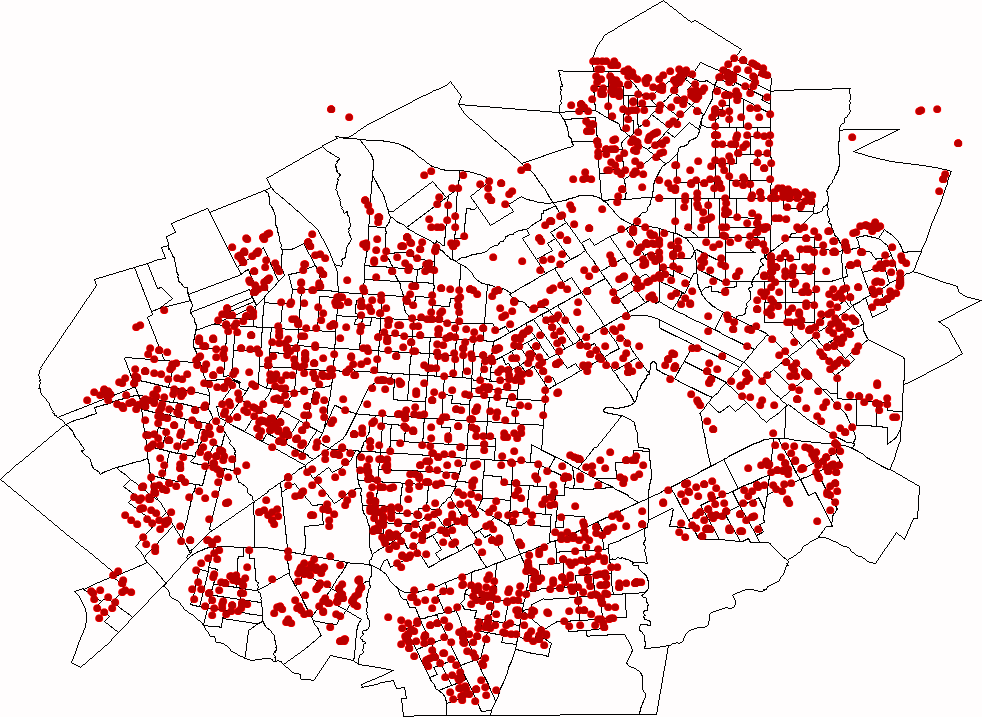
\includegraphics[width=1.0\textwidth]{Figuras/Resultados/Observado/01-09-2009.png}
    \captionsetup{labelformat=empty}
    \captionof{figure}{Dia 1 de Setembro de 2009}
  \end{minipage}%
  \centering
  \begin{minipage}{.45\textwidth}
    \centering
    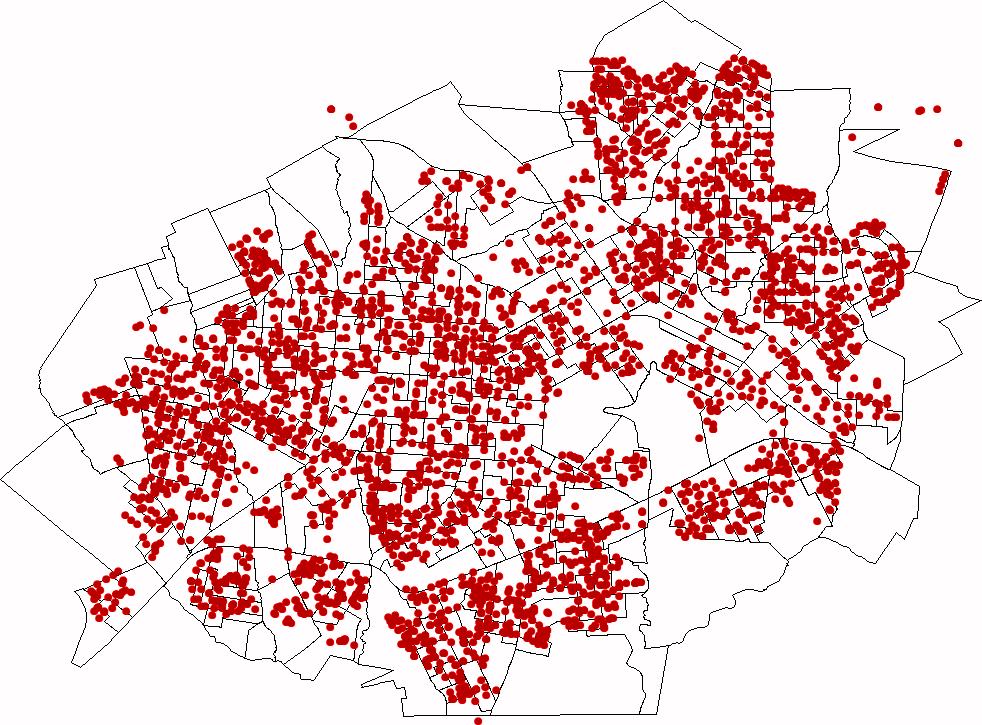
\includegraphics[width=1.0\textwidth]{Figuras/Resultados/Observado/01-10-2009.png}
    \captionsetup{labelformat=empty}
    \captionof{figure}{Dia 1 de Outubro de 2009}
  \end{minipage}
  \begin{minipage}{.45\textwidth}
    \centering
    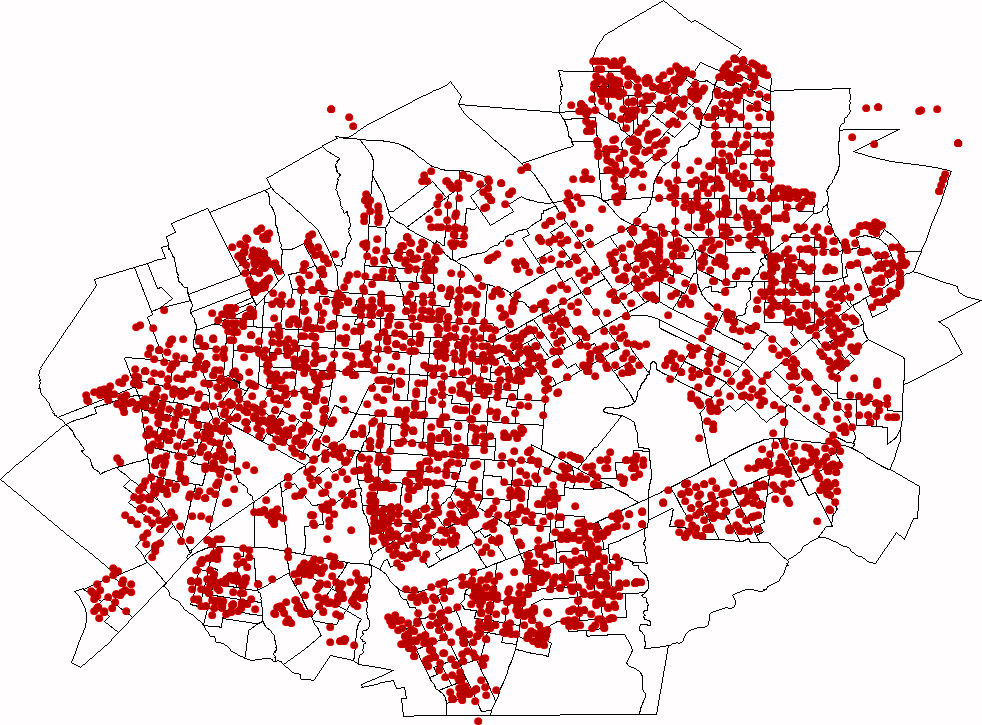
\includegraphics[width=1.0\textwidth]{Figuras/Resultados/Observado/01-11-2009.png}
    \captionsetup{labelformat=empty}
    \captionof{figure}{Dia 1 de Novembro de 2009}
  \end{minipage}%
  \begin{minipage}{.45\textwidth}
    \centering
    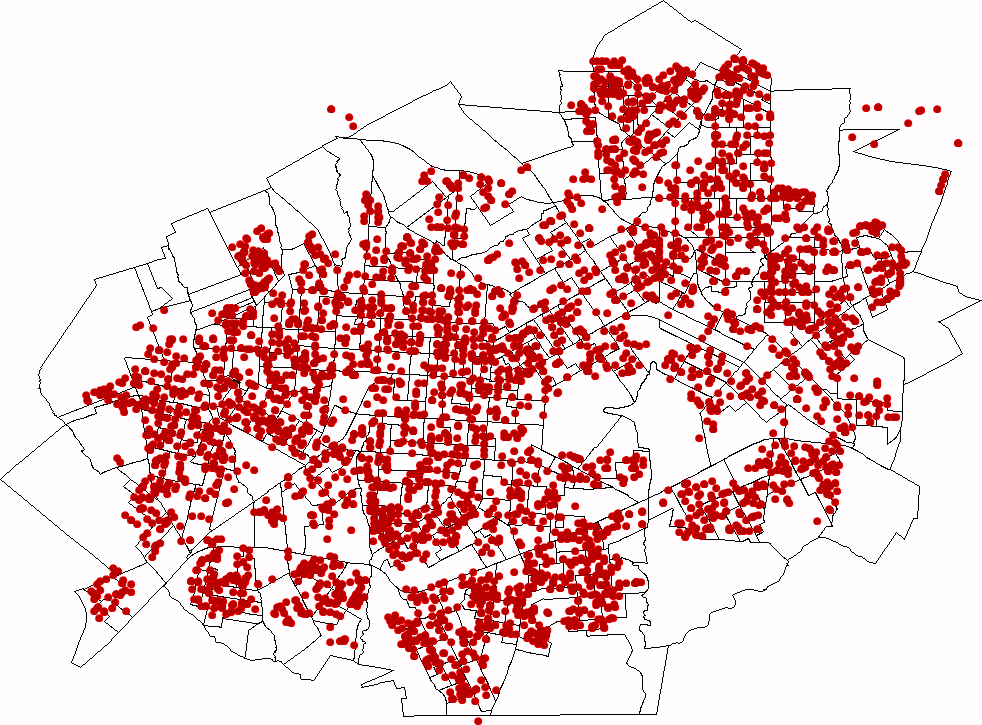
\includegraphics[width=1.0\textwidth]{Figuras/Resultados/Observado/01-12-2009.png}
    \captionsetup{labelformat=empty}
    \captionof{figure}{Dia 1 de Dezembro de 2009}
  \end{minipage}
  \caption{Espalhamento espacial observados dos casos de Influenza.}
  \label{fig:espacial_observado_0002}
\end{figure}

\newpage
